% Options for packages loaded elsewhere
% Options for packages loaded elsewhere
\PassOptionsToPackage{unicode,draft}{hyperref}
\PassOptionsToPackage{hyphens}{url}
\PassOptionsToPackage{dvipsnames,svgnames,x11names}{xcolor}
%
\documentclass[
  11pt,
  letterpaper,
  DIV=11,
  numbers=noendperiod]{scrartcl}
\usepackage{xcolor}
\usepackage[landscape,margin=0.8in]{geometry}
\usepackage{amsmath,amssymb}
\setcounter{secnumdepth}{5}
\usepackage{iftex}
\ifPDFTeX
  \usepackage[T1]{fontenc}
  \usepackage[utf8]{inputenc}
  \usepackage{textcomp} % provide euro and other symbols
\else % if luatex or xetex
  \usepackage{unicode-math} % this also loads fontspec
  \defaultfontfeatures{Scale=MatchLowercase}
  \defaultfontfeatures[\rmfamily]{Ligatures=TeX,Scale=1}
\fi
\usepackage{lmodern}
\ifPDFTeX\else
  % xetex/luatex font selection
  \setmainfont[]{Latin Modern Roman}
\fi
% Use upquote if available, for straight quotes in verbatim environments
\IfFileExists{upquote.sty}{\usepackage{upquote}}{}
\IfFileExists{microtype.sty}{% use microtype if available
  \usepackage[]{microtype}
  \UseMicrotypeSet[protrusion]{basicmath} % disable protrusion for tt fonts
}{}
\makeatletter
\@ifundefined{KOMAClassName}{% if non-KOMA class
  \IfFileExists{parskip.sty}{%
    \usepackage{parskip}
  }{% else
    \setlength{\parindent}{0pt}
    \setlength{\parskip}{6pt plus 2pt minus 1pt}}
}{% if KOMA class
  \KOMAoptions{parskip=half}}
\makeatother
% Make \paragraph and \subparagraph free-standing
\makeatletter
\ifx\paragraph\undefined\else
  \let\oldparagraph\paragraph
  \renewcommand{\paragraph}{
    \@ifstar
      \xxxParagraphStar
      \xxxParagraphNoStar
  }
  \newcommand{\xxxParagraphStar}[1]{\oldparagraph*{#1}\mbox{}}
  \newcommand{\xxxParagraphNoStar}[1]{\oldparagraph{#1}\mbox{}}
\fi
\ifx\subparagraph\undefined\else
  \let\oldsubparagraph\subparagraph
  \renewcommand{\subparagraph}{
    \@ifstar
      \xxxSubParagraphStar
      \xxxSubParagraphNoStar
  }
  \newcommand{\xxxSubParagraphStar}[1]{\oldsubparagraph*{#1}\mbox{}}
  \newcommand{\xxxSubParagraphNoStar}[1]{\oldsubparagraph{#1}\mbox{}}
\fi
\makeatother

\usepackage{color}
\usepackage{fancyvrb}
\newcommand{\VerbBar}{|}
\newcommand{\VERB}{\Verb[commandchars=\\\{\}]}
\DefineVerbatimEnvironment{Highlighting}{Verbatim}{commandchars=\\\{\}}
% Add ',fontsize=\small' for more characters per line
\usepackage{framed}
\definecolor{shadecolor}{RGB}{241,243,245}
\newenvironment{Shaded}{\begin{snugshade}}{\end{snugshade}}
\newcommand{\AlertTok}[1]{\textcolor[rgb]{0.68,0.00,0.00}{#1}}
\newcommand{\AnnotationTok}[1]{\textcolor[rgb]{0.37,0.37,0.37}{#1}}
\newcommand{\AttributeTok}[1]{\textcolor[rgb]{0.40,0.45,0.13}{#1}}
\newcommand{\BaseNTok}[1]{\textcolor[rgb]{0.68,0.00,0.00}{#1}}
\newcommand{\BuiltInTok}[1]{\textcolor[rgb]{0.00,0.23,0.31}{#1}}
\newcommand{\CharTok}[1]{\textcolor[rgb]{0.13,0.47,0.30}{#1}}
\newcommand{\CommentTok}[1]{\textcolor[rgb]{0.37,0.37,0.37}{#1}}
\newcommand{\CommentVarTok}[1]{\textcolor[rgb]{0.37,0.37,0.37}{\textit{#1}}}
\newcommand{\ConstantTok}[1]{\textcolor[rgb]{0.56,0.35,0.01}{#1}}
\newcommand{\ControlFlowTok}[1]{\textcolor[rgb]{0.00,0.23,0.31}{\textbf{#1}}}
\newcommand{\DataTypeTok}[1]{\textcolor[rgb]{0.68,0.00,0.00}{#1}}
\newcommand{\DecValTok}[1]{\textcolor[rgb]{0.68,0.00,0.00}{#1}}
\newcommand{\DocumentationTok}[1]{\textcolor[rgb]{0.37,0.37,0.37}{\textit{#1}}}
\newcommand{\ErrorTok}[1]{\textcolor[rgb]{0.68,0.00,0.00}{#1}}
\newcommand{\ExtensionTok}[1]{\textcolor[rgb]{0.00,0.23,0.31}{#1}}
\newcommand{\FloatTok}[1]{\textcolor[rgb]{0.68,0.00,0.00}{#1}}
\newcommand{\FunctionTok}[1]{\textcolor[rgb]{0.28,0.35,0.67}{#1}}
\newcommand{\ImportTok}[1]{\textcolor[rgb]{0.00,0.46,0.62}{#1}}
\newcommand{\InformationTok}[1]{\textcolor[rgb]{0.37,0.37,0.37}{#1}}
\newcommand{\KeywordTok}[1]{\textcolor[rgb]{0.00,0.23,0.31}{\textbf{#1}}}
\newcommand{\NormalTok}[1]{\textcolor[rgb]{0.00,0.23,0.31}{#1}}
\newcommand{\OperatorTok}[1]{\textcolor[rgb]{0.37,0.37,0.37}{#1}}
\newcommand{\OtherTok}[1]{\textcolor[rgb]{0.00,0.23,0.31}{#1}}
\newcommand{\PreprocessorTok}[1]{\textcolor[rgb]{0.68,0.00,0.00}{#1}}
\newcommand{\RegionMarkerTok}[1]{\textcolor[rgb]{0.00,0.23,0.31}{#1}}
\newcommand{\SpecialCharTok}[1]{\textcolor[rgb]{0.37,0.37,0.37}{#1}}
\newcommand{\SpecialStringTok}[1]{\textcolor[rgb]{0.13,0.47,0.30}{#1}}
\newcommand{\StringTok}[1]{\textcolor[rgb]{0.13,0.47,0.30}{#1}}
\newcommand{\VariableTok}[1]{\textcolor[rgb]{0.07,0.07,0.07}{#1}}
\newcommand{\VerbatimStringTok}[1]{\textcolor[rgb]{0.13,0.47,0.30}{#1}}
\newcommand{\WarningTok}[1]{\textcolor[rgb]{0.37,0.37,0.37}{\textit{#1}}}

\usepackage{longtable,booktabs,array}
\usepackage{calc} % for calculating minipage widths
% Correct order of tables after \paragraph or \subparagraph
\usepackage{etoolbox}
\makeatletter
\patchcmd\longtable{\par}{\if@noskipsec\mbox{}\fi\par}{}{}
\makeatother
% Allow footnotes in longtable head/foot
\IfFileExists{footnotehyper.sty}{\usepackage{footnotehyper}}{\usepackage{footnote}}
\makesavenoteenv{longtable}
\usepackage{graphicx}
\makeatletter
\newsavebox\pandoc@box
\newcommand*\pandocbounded[1]{% scales image to fit in text height/width
  \sbox\pandoc@box{#1}%
  \Gscale@div\@tempa{\textheight}{\dimexpr\ht\pandoc@box+\dp\pandoc@box\relax}%
  \Gscale@div\@tempb{\linewidth}{\wd\pandoc@box}%
  \ifdim\@tempb\p@<\@tempa\p@\let\@tempa\@tempb\fi% select the smaller of both
  \ifdim\@tempa\p@<\p@\scalebox{\@tempa}{\usebox\pandoc@box}%
  \else\usebox{\pandoc@box}%
  \fi%
}
% Set default figure placement to htbp
\def\fps@figure{htbp}
\makeatother





\setlength{\emergencystretch}{3em} % prevent overfull lines

\providecommand{\tightlist}{%
  \setlength{\itemsep}{0pt}\setlength{\parskip}{0pt}}



 


\usepackage{fvextra}
\definecolor{codebgcolor}{HTML}{F6F8FA}
\fvset{breaklines=true,breakanywhere=true}
\DefineVerbatimEnvironment{Highlighting}{Verbatim}{commandchars=\\\{\},breaklines,breakanywhere,bgcolor=codebgcolor}
\makeatletter
\@ifundefined{Shaded}{%
  \newenvironment{Shaded}{}{}%
}{%
  \renewenvironment{Shaded}{}{}%
}
\makeatother
\usepackage{booktabs}
\usepackage{longtable}
\usepackage{array}
\usepackage{multirow}
\usepackage{wrapfig}
\usepackage{float}
\usepackage{colortbl}
\usepackage{pdflscape}
\usepackage{tabu}
\usepackage{threeparttable}
\usepackage{threeparttablex}
\usepackage[normalem]{ulem}
\usepackage{makecell}
\usepackage{xcolor}
\usepackage{caption}
\usepackage{anyfontsize}
\KOMAoption{captions}{tableheading}
\usepackage{float}
\usepackage{placeins}
\graphicspath{{../}{./}}
\makeatletter
\@ifpackageloaded{caption}{}{\usepackage{caption}}
\AtBeginDocument{%
\ifdefined\contentsname
  \renewcommand*\contentsname{Table of contents}
\else
  \newcommand\contentsname{Table of contents}
\fi
\ifdefined\listfigurename
  \renewcommand*\listfigurename{List of Figures}
\else
  \newcommand\listfigurename{List of Figures}
\fi
\ifdefined\listtablename
  \renewcommand*\listtablename{List of Tables}
\else
  \newcommand\listtablename{List of Tables}
\fi
\ifdefined\figurename
  \renewcommand*\figurename{Figure}
\else
  \newcommand\figurename{Figure}
\fi
\ifdefined\tablename
  \renewcommand*\tablename{Table}
\else
  \newcommand\tablename{Table}
\fi
}
\@ifpackageloaded{float}{}{\usepackage{float}}
\floatstyle{ruled}
\@ifundefined{c@chapter}{\newfloat{codelisting}{h}{lop}}{\newfloat{codelisting}{h}{lop}[chapter]}
\floatname{codelisting}{Listing}
\newcommand*\listoflistings{\listof{codelisting}{List of Listings}}
\makeatother
\makeatletter
\makeatother
\makeatletter
\@ifpackageloaded{caption}{}{\usepackage{caption}}
\@ifpackageloaded{subcaption}{}{\usepackage{subcaption}}
\makeatother
\usepackage{bookmark}
\IfFileExists{xurl.sty}{\usepackage{xurl}}{} % add URL line breaks if available
\urlstyle{same}
\hypersetup{
  pdftitle={ABG‑VBG Analysis},
  pdfauthor={Brian Locke, Anila Mehta},
  colorlinks=true,
  linkcolor={blue},
  filecolor={Maroon},
  citecolor={Blue},
  urlcolor={Blue},
  pdfcreator={LaTeX via pandoc}}


\title{ABG‑VBG Analysis}
\author{Brian Locke, Anila Mehta}
\date{}
\begin{document}
\maketitle

\renewcommand*\contentsname{Table of contents}
{
\hypersetup{linkcolor=}
\setcounter{tocdepth}{3}
\tableofcontents
}

\begin{Shaded}
\begin{Highlighting}[]
\CommentTok{\# }\AlertTok{TODO}\CommentTok{ (future work):}
\CommentTok{\# P1: ABG residual imbalance \textgreater{}0.10 — consider redefining target population / stratified standardization / overlap restriction.}
\CommentTok{\# P3: Separation/nonconvergence in adjusted outcome models — consider penalized logistic / level collapsing, and define reporting policy.}
\CommentTok{\# }\AlertTok{TODO}\CommentTok{ consider adding discontinuity (at 45 mmHg CO2 on ABG and 50 mmHg CO2 on VBG; start with raw binning and LOESS to evaluate if there\textquotesingle{}s a jump, then consider regression discontinuity or similar if so).}
\end{Highlighting}
\end{Shaded}

\section{Data Pre-Processing and Unweighted
Analyses}\label{data-pre-processing-and-unweighted-analyses}

This code pulls in the master database (a STATA file) and does some
initial cleaning - this will only need to be run once, and then the data
can be accessed in the usual way.

Package dependencies are managed via \texttt{renv} for reproducibility.
Use \texttt{renv::restore()} before rendering.

\subsubsection{Package Set Up}\label{package-set-up}

\subsection{Helper functions for model
diagnostics}\label{helper-functions-for-model-diagnostics}

\begin{center}\textbf{Seed escrow for MI and GBM runs}\end{center}

\begin{table}[!h]
\centering\begingroup\fontsize{7}{9}\selectfont

\resizebox{\ifdim\width>\linewidth\linewidth\else\width\fi}{!}{
\begin{tabular}{ll}
\toprule
component & seed\\
\midrule
Multiple imputation (mice) & 20251206\\
ABG propensity GBM (non-MI) & 42\\
VBG propensity GBM (non-MI) & 42\\
MI PS (glm RCS) seeds (ABG per imputation) & 20251206 + imputation index\\
MI PS (glm RCS) seeds (VBG per imputation) & 30251206 + imputation index\\
\bottomrule
\end{tabular}}
\endgroup{}
\end{table}

Converts the data from a STATA format to rdata if the rdata file does
not exist. If it does already exist, it just loads that.

\subsubsection{Configuration for the IPW
models}\label{configuration-for-the-ipw-models}

\begin{landscape}

\begin{center}\textbf{Run metadata (pilot vs full)}\end{center}

\begin{table}[!h]
\centering\begingroup\fontsize{7}{9}\selectfont

\resizebox{\ifdim\width>\linewidth\linewidth\else\width\fi}{!}{
\begin{tabular}{llrrlr}
\toprule
run\_id & run\_mode & pilot\_frac & mi\_ram\_gb & mi\_ram\_gb\_source & mi\_batch\_threshold\\
\midrule
20260424\_063653 & pilot & 0.01 & 16 & auto:Darwin & 5000\\
\bottomrule
\end{tabular}}
\endgroup{}
\end{table}

\begin{table}[!h]
\centering\begingroup\fontsize{7}{9}\selectfont

\resizebox{\ifdim\width>\linewidth\linewidth\else\width\fi}{!}{
\begin{tabular}{rlrrr}
\toprule
mi\_batch\_start & mi\_batch\_start\_source & full\_n & sampled\_n & subset\_n\\
\midrule
2 & auto:auto:Darwin & 833476 & 8335 & 5175\\
\bottomrule
\end{tabular}}
\endgroup{}
\end{table}

\end{landscape}

Codebook artifact path: Results/codebookr.docx. Generation is skipped in
pilot mode to keep notebook validation renders fast.

\subsubsection{Outcome Variable
Creation}\label{outcome-variable-creation}

\subsection{Baseline tables}\label{baseline-tables}

\FloatBarrier\nopagebreak

\par

\noindent

\FloatBarrier\nopagebreak

\par

\noindent

\FloatBarrier\nopagebreak

\par

\noindent

\subsection{Three-level PCO2 categories
(unweighted)}\label{three-level-pco2-categories-unweighted}

Three groups using low/normal/high CO2 categories

\subsection{Observed outcome rates by CO2 bin
(unweighted)}\label{observed-outcome-rates-by-co2-bin-unweighted}

\subsection{Restricted cubic spline regressions
(unweighted)}\label{restricted-cubic-spline-regressions-unweighted}

Spline curves are shown as odds ratios relative to CO2\_ref (midpoint of
the normal range), holding covariates at the reference profile.

\subsubsection{Unweighted, Restricted Cubic Spline Regression - ABG by
PaCO2}\label{unweighted-restricted-cubic-spline-regression---abg-by-paco2}

\subsubsection{Unweighted, Restricted Cubic Spline -
VBG}\label{unweighted-restricted-cubic-spline---vbg}

\FloatBarrier\nopagebreak

\par

\noindent

\section{Inverse Propensity Weighting
(GBM)}\label{inverse-propensity-weighting-gbm}

IPW done using Gradient Boosting Methods (GBM) - a type of decision-tree
based machine learning. ``\textbf{\emph{Random forests and GBM are
designed to automatically include relevant interactions for variables
included in the model.}} As such, using a GBM to estimate the PS model,
can reduce model misspecification, since \textbf{\emph{the analyst is
not required to identify relevant interactions or nonlinearities.''}}
from this citation: PMID:
\href{https://pubmed.ncbi.nlm.nih.gov/39947224/}{39947224}. PMCID:
\href{https://pmc.ncbi.nlm.nih.gov/articles/PMC11825193/}{PMC11825193}.

Current propensity score uses \texttt{covars\_gbm} (demographics,
comorbidities, encounter type, vitals, labs) as defined above; in this
block only \texttt{encounter\_type} is explicitly factored before
weighting.

Note: for all these, I suggested new GBM adjustments that accomplish the
following:

\begin{enumerate}
\def\labelenumi{\arabic{enumi}.}
\item
  Smaller GBM \& balance‑based stopping (stop.method = ``smd.max'') →
  faster fit, avoids over‑fitting, lighter tails (which lead to extreme
  weights that are problematic).
\item
  Target balance compares weighted treated cohort to the full sample;
  aim for \textbar SMD\textbar{} \textless{} 0.1.
\item
  Weight stabilization (divide by mean) mitigates a few huge weights. We
  use one‑sided truncation at very small propensities (caps large
  weights only).
\item
  Uses robust variance estimation (e.g.~allows the variances to change
  by PaCO2) for IP‑weighted GLM; works with splines via rcs(). This is a
  bit nuanced but I think good to change even though it adds complexity
\item
  Deterministic seed ensures result replication.
\end{enumerate}

\subsubsection{ABG IPW weighting and
diagnostics}\label{abg-ipw-weighting-and-diagnostics}

GBM tuning is shared across ABG and VBG via \texttt{gbm\_params} to keep
symmetry; update there if needed.

\textbf{Inverse Propensity-Weighted Logistic Regressions with CO2
predictor represented as a restricted cubic spline.}

These are covariate-adjusted outcome models (outcome \textasciitilde{}
spline(CO2) + X), fit separately for ABG and VBG cohorts using
survey::svyglm with robust (design-based) SEs. Spline curves are shown
as odds ratios relative to CO2\_ref (midpoint of the normal range).

\subsubsection{ABG IPW spline models}\label{abg-ipw-spline-models}

Restricting plots bewtween 0.02 and 0.98

\subsubsection{ABG IPW spline models (2--98th
percentile)}\label{abg-ipw-spline-models-298th-percentile}

VBG uses the same GBM tuning as ABG (shared \texttt{gbm\_params}).

\subsubsection{VBG IPW weighting and spline
models}\label{vbg-ipw-weighting-and-spline-models}

\subsubsection{Three-level PCO2 categories (weighted; ABG,
VBG)}\label{three-level-pco2-categories-weighted-abg-vbg}

Three groups with weights and covariate adjustment

\subsubsection{Observed outcome rates by CO2 bin (GBM IPSW,
non-MI)}\label{observed-outcome-rates-by-co2-bin-gbm-ipsw-non-mi}

\subsection{Propensity score
diagnostics}\label{propensity-score-diagnostics}

Plotting propensity scores

\pandocbounded{
\includegraphics[keepaspectratio]{Results/figs/propensity-histograms-all-1.png}}

\section{Multiple Imputation (and logistic
IPSW)}\label{multiple-imputation-and-logistic-ipsw}

added 12/6/2025

\subsubsection{Missingness structure and
drivers}\label{missingness-structure-and-drivers}

\FloatBarrier\nopagebreak

\par

\noindent

\subsubsection{Monte Carlo error check after
MI}\label{monte-carlo-error-check-after-mi}

\subsection{Pre‑imputation data prep (consistent types \&
predictors)}\label{preimputation-data-prep-consistent-types-predictors}

\textbf{Why}: MI models need coherent types; using exactly the same
covariates as the propensity score models avoids model drift.

\subsection{Imputation model specification
(MICE)}\label{imputation-model-specification-mice}

\subsubsection{Predictor matrix \& methods. Run MICE (moderate settings
for
scale)}\label{predictor-matrix-methods.-run-mice-moderate-settings-for-scale}

\subsection{Refit propensity models within each
imputation}\label{refit-propensity-models-within-each-imputation}

MI propensity scores use logistic regression with restricted cubic
splines (\texttt{rms::rcs}, 4 knots by default) for continuous
covariates; the same covariate set used in non‑MI models is reused here
(\texttt{covars\_ps}). IPSW truncation rules are unchanged.

Note: the MI computations below run in a single pass per imputation
(weights, balance, cat3, spline). Subsequent MI sections reuse those
outputs and will stop if they are missing.

\subsubsection{FAIL-FAST CHECKS}\label{fail-fast-checks}

\begin{verbatim}
            used   (Mb) gc trigger   (Mb) limit (Mb)  max used   (Mb)
Ncells   7084799  378.4   11855017  633.2         NA  11855017  633.2
Vcells 485113151 3701.2  964751313 7360.5      16384 964680566 7360.0
\end{verbatim}

\begin{verbatim}
[1] TRUE
\end{verbatim}

\subsubsection{ABG propensity (has\_abg)}\label{abg-propensity-has_abg}

\subsubsection{Balance diagnostics across
imputations}\label{balance-diagnostics-across-imputations}

\subsubsection{VBG propensity (has\_vbg)}\label{vbg-propensity-has_vbg}

\subsubsection{VBG balance}\label{vbg-balance}

\subsection{Weighted outcome models within each imputation +
pooling}\label{weighted-outcome-models-within-each-imputation-pooling}

Within each imputation, fit covariate‑adjusted CO2 spline outcome models
\textbf{only in the measured cohort} (has\_abg==1 for PaCO2; has\_vbg==1
for VBG CO2), using IPSW weights to address nonrandom testing. Curves
are pooled pointwise across imputations (Rubin's rules on the log‑OR
scale) and displayed as odds ratios relative to CO2\_ref at a reference
covariate profile.

\subsubsection{Helper: fit + extract log‑OR and SE from
svyglm}\label{helper-fit-extract-logor-and-se-from-svyglm}

\subsubsection{VBG: MI pooled spline models (treated cohort
only)}\label{vbg-mi-pooled-spline-models-treated-cohort-only}

\subsection{Explainability}\label{explainability}

\subsection{MI three‑level PCO2 helpers and
checks}\label{mi-threelevel-pco2-helpers-and-checks}

\subsection{MI + IPW three-level PCO2 (ABG \&
VBG)}\label{mi-ipw-three-level-pco2-abg-vbg}

\subsubsection{ABG: MI + IPW, three-level PCO2
outcomes}\label{abg-mi-ipw-three-level-pco2-outcomes}

\subsubsection{VBG: MI + IPW, three-level PCO2
outcomes}\label{vbg-mi-ipw-three-level-pco2-outcomes}

\subsubsection{MI-pooled IPW associations (3-level
CO2)}\label{mi-pooled-ipw-associations-3-level-co2}

\begin{table}
\caption*{
{\fontsize{20}{25}\selectfont  MI-pooled MI-logistic IPSW associations between CO2 category and outcomes (adjusted)\fontsize{12}{15}\selectfont }
} 
\fontsize{12.0pt}{14.0pt}\selectfont
\begin{tabular*}{\linewidth}{@{\extracolsep{\fill}}llrr}
\toprule
Cohort & Outcome & Low vs normal OR (95\% CI) & High vs normal OR (95\% CI) \\ 
\midrule\addlinespace[2.5pt]
ABG & IMV & 1.41 (1.05, 1.90) & 1.26 (0.93, 1.71) \\ 
VBG & IMV & 1.24 (0.77, 2.00) & 1.63 (1.02, 2.60) \\ 
ABG & NIV & 1.04 (0.63, 1.72) & 3.05 (1.99, 4.68) \\ 
VBG & NIV & 0.76 (0.38, 1.52) & 2.69 (1.47, 4.90) \\ 
ABG & Death (60d) & 1.55 (1.07, 2.25) & 1.50 (1.06, 2.14) \\ 
VBG & Death (60d) & 1.10 (0.68, 1.79) & 1.10 (0.70, 1.74) \\ 
ABG & Hypercapnic RF & 1.26 (0.70, 2.26) & 9.21 (5.73, 14.81) \\ 
VBG & Hypercapnic RF & 0.68 (0.30, 1.54) & 6.28 (3.50, 11.25) \\ 
\bottomrule
\end{tabular*}
\begin{minipage}{\linewidth}
\vspace{.05em}
Weighted survey GLMs adjusted for baseline covariates; weights = MI-specific GLM (RCS) IPW; m = 20 imputations (seed 20251206); reference = Normal.\\
\end{minipage}
\end{table}

\subsubsection{Summary: adjusted CO2-category associations across
analysis
tracks}\label{summary-adjusted-co2-category-associations-across-analysis-tracks}

\subsection{Canonical Categorical Key-Results Figures Across Analysis
Tracks}\label{canonical-categorical-key-results-figures-across-analysis-tracks}

\subsection{Observed outcome rates by CO2 bin (MI-logistic
IPSW)}\label{observed-outcome-rates-by-co2-bin-mi-logistic-ipsw}

\subsection{Manuscript outputs
summary}\label{manuscript-outputs-summary}

\begin{verbatim}

TRUE 
  20 
\end{verbatim}

\subsubsection{Visualization: pooled three-level
ORs}\label{visualization-pooled-three-level-ors}

\subsubsection{Visualization: pooled three-level predicted
probabilities}\label{visualization-pooled-three-level-predicted-probabilities}

\FloatBarrier\nopagebreak

\par

\noindent

\subsubsection{Visualization}\label{visualization}

\subsection{Canonical Key-Results Figures Across Analysis
Tracks}\label{canonical-key-results-figures-across-analysis-tracks}

The following 4×2 figures are the canonical manuscript-facing spline
displays across crude, adjusted, imputed, and weighted analyses.

\FloatBarrier\nopagebreak

\par

\noindent

\section{Diagnostics and Exports}\label{diagnostics-and-exports}

\subsubsection{MI convergence and
mixing}\label{mi-convergence-and-mixing}

\begin{verbatim}
png 
  2 
\end{verbatim}

\subsubsection{MI stability across m}\label{mi-stability-across-m}

\subsubsection{MI maxit sensitivity
(sampled)}\label{mi-maxit-sensitivity-sampled}

\subsubsection{Balance diagnostics}\label{balance-diagnostics}

\subsubsection{Outcome diagnostics}\label{outcome-diagnostics}

\subsubsection{Diagnostics summary and
audit}\label{diagnostics-summary-and-audit}

\subsubsection{Warning and model-fit
diagnostics}\label{warning-and-model-fit-diagnostics}

\subsubsection{Notebook chunk runtime
log}\label{notebook-chunk-runtime-log}

\section{Analysis of the discordance between predicted probabilities and
OR for NIV and
IMV}\label{analysis-of-the-discordance-between-predicted-probabilities-and-or-for-niv-and-imv}

This section is diagnostic and additive. It does not change the primary
manuscript estimates; instead it reproduces the NIV/IMV probability-OR
discordance and checks whether it is explained by reference profiles,
probability scale, residual capture/missingness, sentinel procedure
capture, support, setting/site, subgroup, or timing structure.

\subsection{Pilot validation and
scope}\label{pilot-validation-and-scope}

\begin{landscape}

\begin{center}\textbf{Current NIV/IMV OR and predicted-probability summaries}\end{center}

\begin{table}[!h]
\centering\begingroup\fontsize{6}{8}\selectfont

\resizebox{\ifdim\width>\linewidth\linewidth\else\width\fi}{!}{
\begin{tabular}{llllrr}
\toprule
Outcome & Modality & Analysis family & CO2 representation & Low vs normal OR & High vs normal OR\\
\midrule
IMV & ABG & MI-logistic IPSW & 3-level category & 1.413 & 1.261\\
IMV & VBG & MI-logistic IPSW & 3-level category & 1.240 & 1.631\\
NIV & ABG & MI-logistic IPSW & 3-level category & 1.042 & 3.049\\
NIV & VBG & MI-logistic IPSW & 3-level category & 0.760 & 2.689\\
IMV & ABG & MI-logistic IPSW & Spline & 1.320 & 1.000\\
\addlinespace
NIV & ABG & MI-logistic IPSW & Spline & 1.046 & 1.371\\
IMV & VBG & MI-logistic IPSW & Spline & 1.033 & 1.089\\
NIV & VBG & MI-logistic IPSW & Spline & 0.966 & 1.475\\
\bottomrule
\end{tabular}}
\endgroup{}
\end{table}

\begin{table}[!h]
\centering\begingroup\fontsize{6}{8}\selectfont

\resizebox{\ifdim\width>\linewidth\linewidth\else\width\fi}{!}{
\begin{tabular}{rrrl}
\toprule
Normal probability & Low probability & High probability & Notes\\
\midrule
0.207 & 0.269 & 0.248 & Current categorical ORs and predicted probabilities.\\
0.193 & 0.228 & 0.280 & Current categorical ORs and predicted probabilities.\\
0.062 & 0.064 & 0.167 & Current categorical ORs and predicted probabilities.\\
0.024 & 0.018 & 0.062 & Current categorical ORs and predicted probabilities.\\
0.200 & 0.248 & 0.200 & Current modality-specific reference profile.\\
\addlinespace
0.063 & 0.066 & 0.084 & Current modality-specific reference profile.\\
0.203 & 0.208 & 0.217 & Current modality-specific reference profile.\\
0.018 & 0.017 & 0.026 & Current modality-specific reference profile.\\
\bottomrule
\end{tabular}}
\endgroup{}
\end{table}

\end{landscape}

{[}1{]} TRUE

\begin{center}
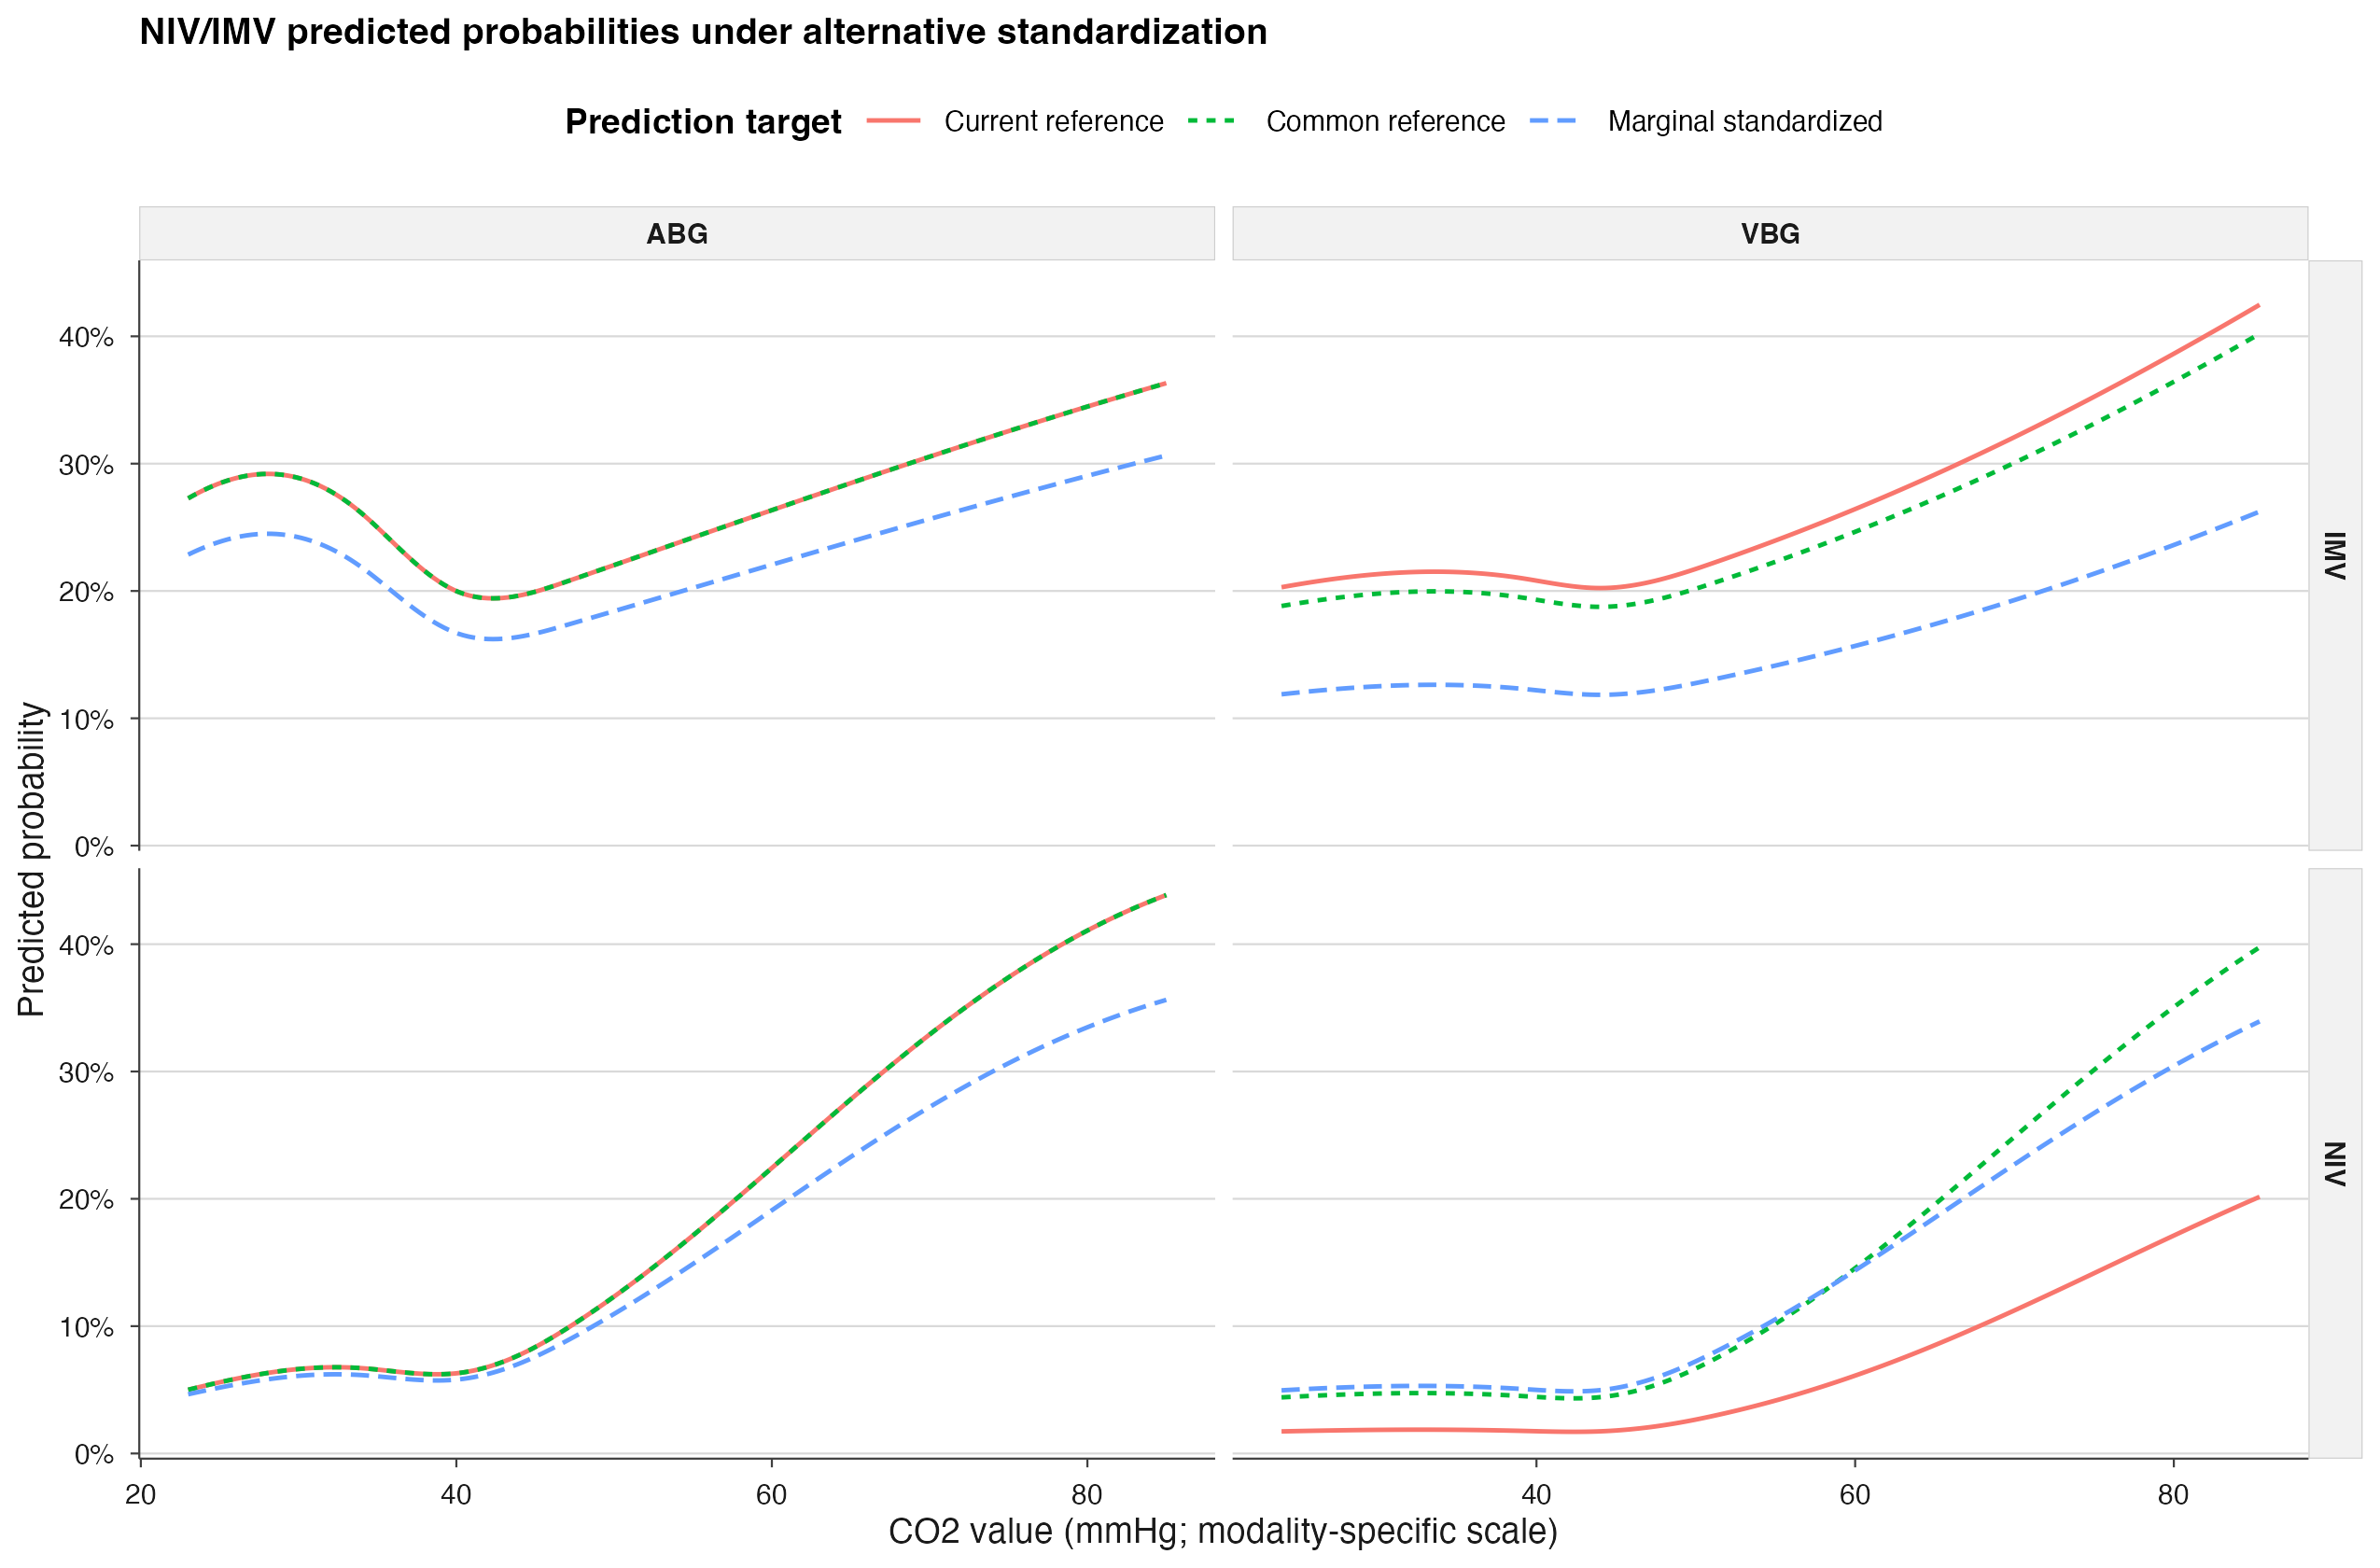
\includegraphics[width=0.94\linewidth,height=0.72\textheight,keepaspectratio]{Results/figs/discordance_probability_standardization_niv_imv.png}
\end{center}

{[}1{]} TRUE

\begin{center}
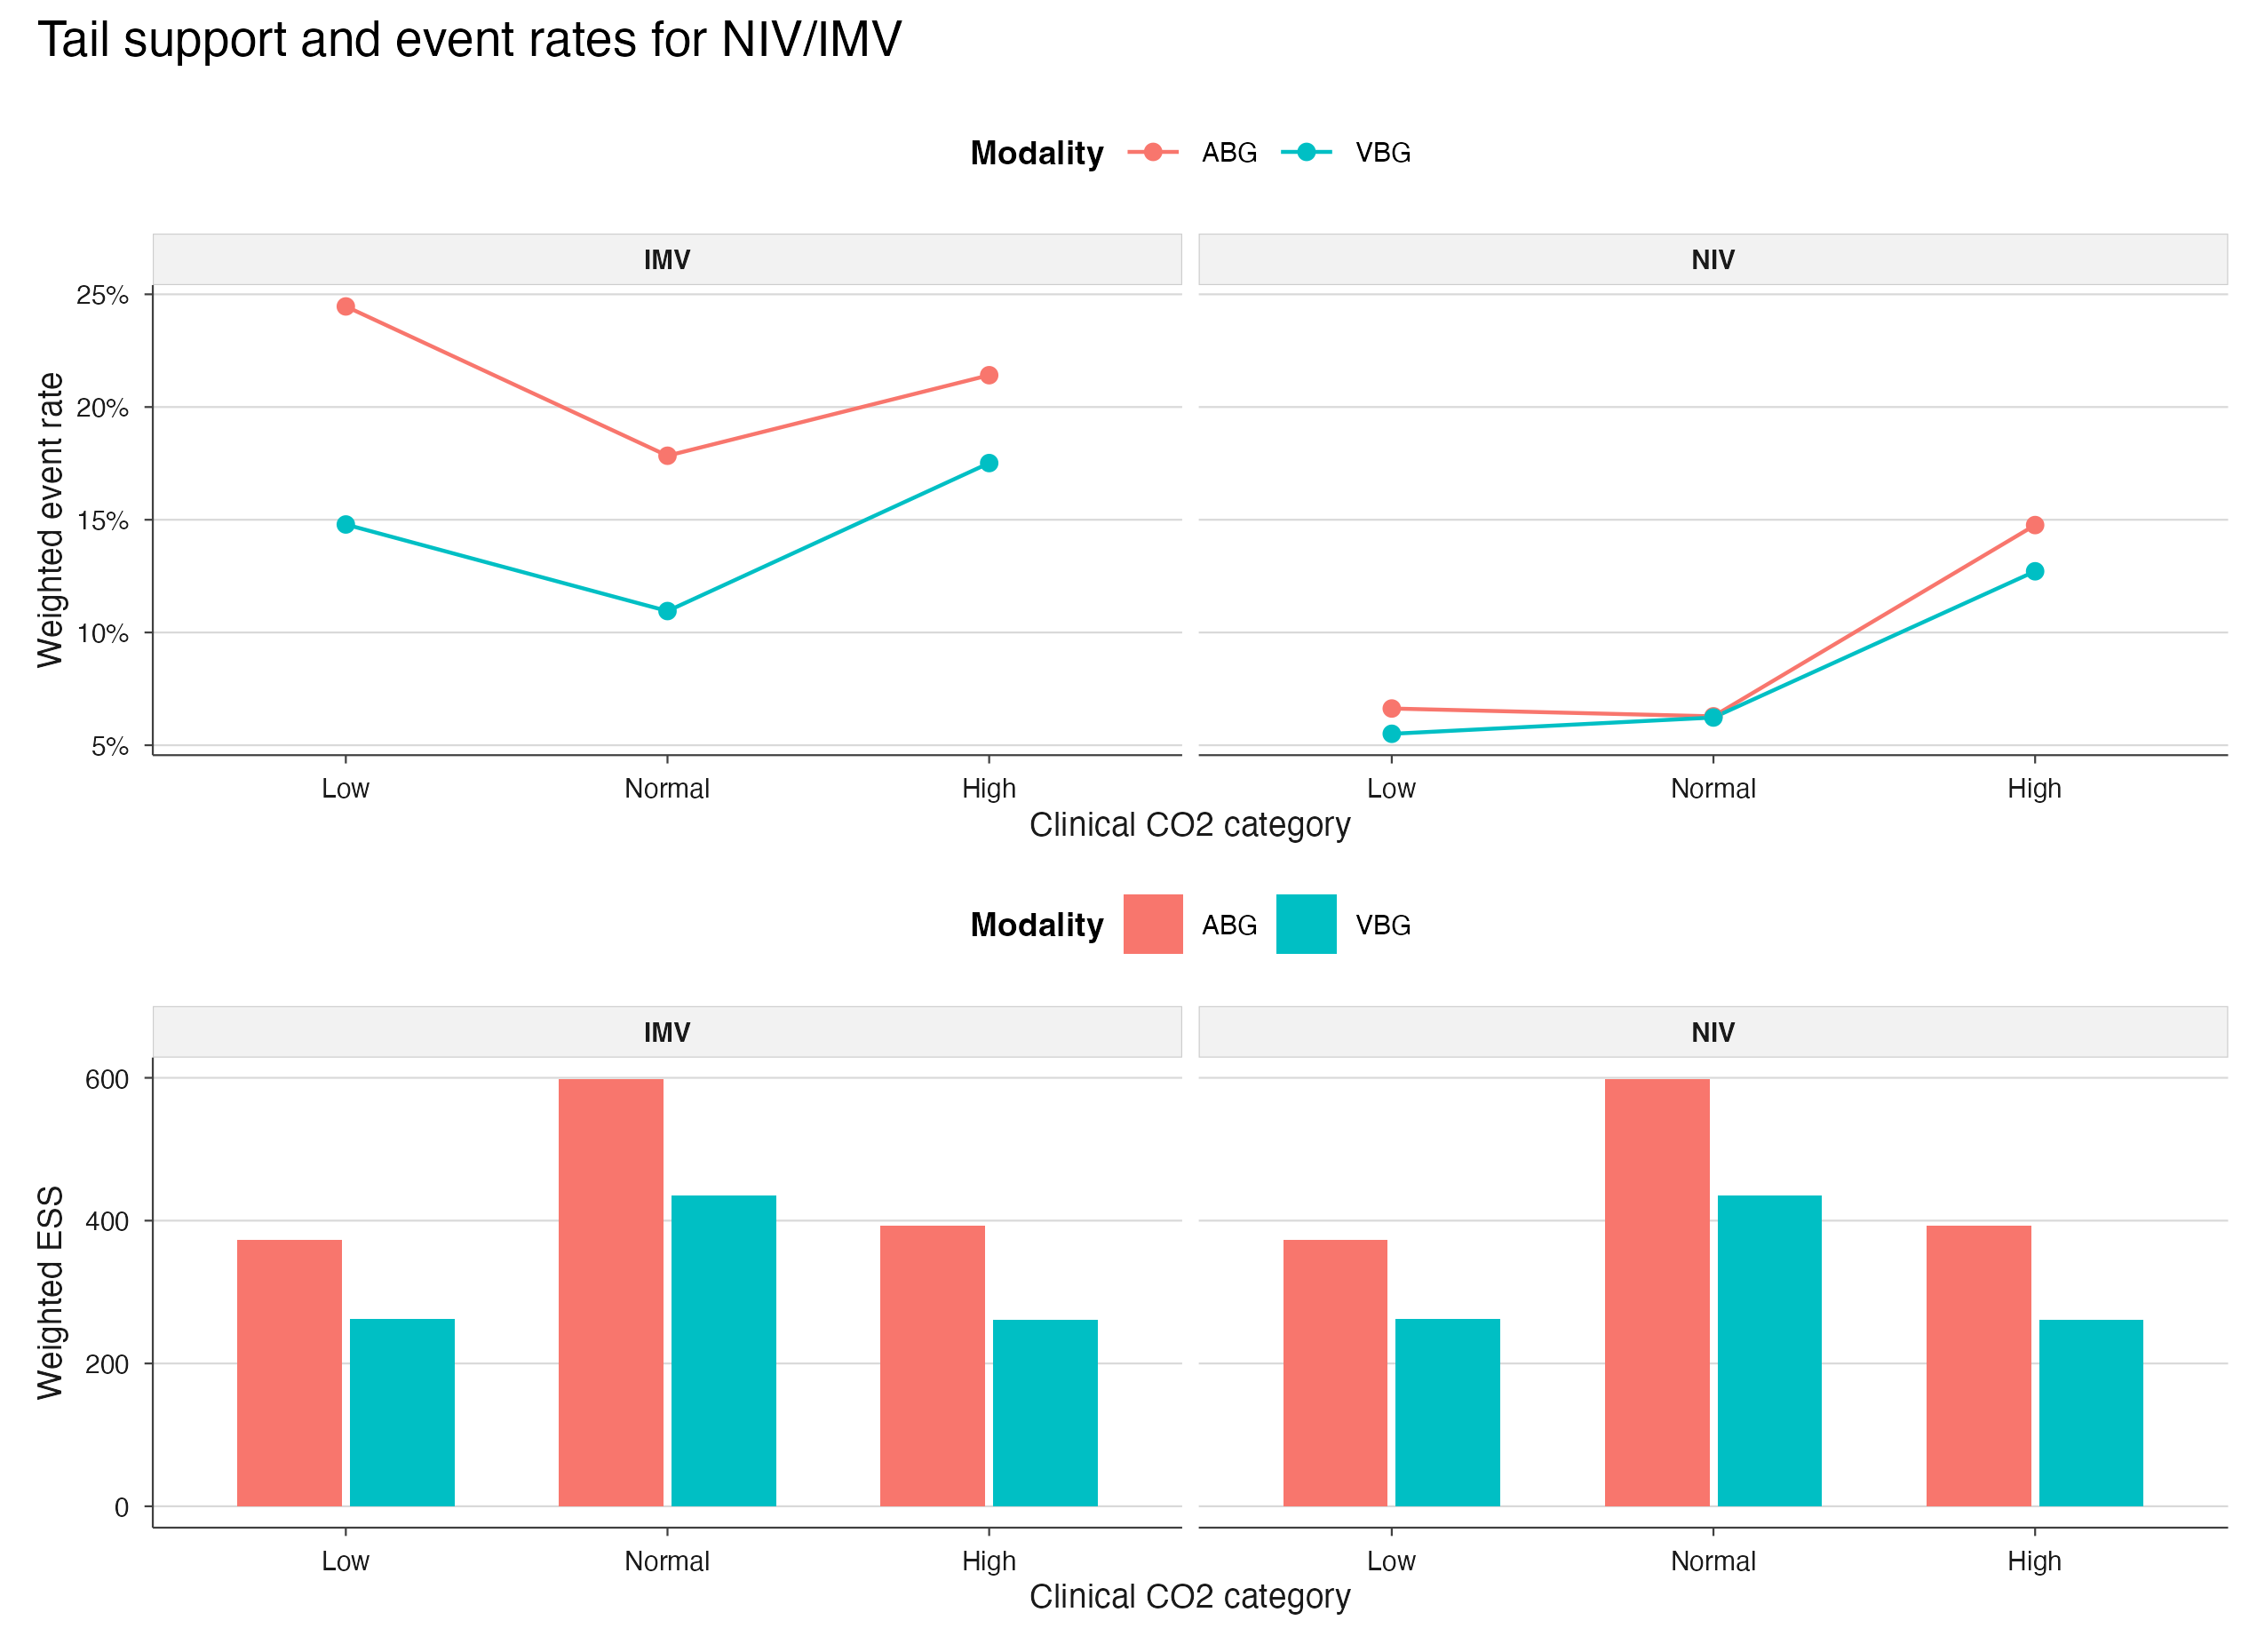
\includegraphics[width=0.94\linewidth,height=0.72\textheight,keepaspectratio]{Results/figs/discordance_tail_support_niv_imv.png}
\end{center}

{[}1{]} TRUE

\begin{landscape}

\begin{center}\textbf{Summary of plausible explanations for NIV/IMV probability-OR discordance}\end{center}

\begin{table}[!h]
\centering\begingroup\fontsize{6}{8}\selectfont

\resizebox{\ifdim\width>\linewidth\linewidth\else\width\fi}{!}{
\begin{tabular}{lllll}
\toprule
Hypothesis & Evidence status & Supported & Not supported & Inconclusive\\
\midrule
Reference-profile / standardization effect & Supported & Yes & No & No\\
Setting or workflow heterogeneity & Supported & Yes & No & No\\
Differential missingness or procedure capture & Partially supported & No & No & No\\
Sentinel procedure capture/completeness & Partially supported & No & No & No\\
Scale / noncollapsibility effect & Not supported & No & Yes & No\\
\addlinespace
Same-encounter timing structure & Not supported & No & Yes & No\\
Tail support / positivity & Supported & Yes & No & No\\
Intrinsic modality-specific measurement effect & Not supported & No & Yes & No\\
\bottomrule
\end{tabular}}
\endgroup{}
\end{table}

\begin{table}[!h]
\centering\begingroup\fontsize{6}{8}\selectfont

\resizebox{\ifdim\width>\linewidth\linewidth\else\width\fi}{!}{
\begin{tabular}{ll}
\toprule
Key evidence & Recommended next step\\
\midrule
Common or marginal standardization shrank at least one current probability gap by >=25\%. & If supported, consider whether manuscript probability curves should use common or marginal standardization in a future methodological ticket.\\
Setting-rate ranges or IMV-focused setting/site diagnostics show material heterogeneity. & If supported, consider setting-stratified or setting-interaction sensitivity models.\\
At least one broad capture/completeness proxy differs, but evidence is not specific enough to prove procedure-capture bias. & If supported, audit NIV/IMV source-field construction and coding-density definitions before changing models.\\
Selected sentinels show some capture/completeness differences, but specificity or directional consistency is insufficient. & If supported, inspect selected sentinel source fields and date-field definitions before attributing NIV/IMV gaps to physiology.\\
OR-scale agreement was not consistently closer than probability-scale agreement. & Use risk differences/RRs beside ORs when communicating procedure outcomes.\\
\addlinespace
Timing-restricted summaries were feasible but did not show a large difference. & If timestamps become available, restrict to blood gases clearly preceding NIV/IMV.\\
At least one clinical/quantile bin had ESS <100 or weighted events <10. & If supported, avoid overinterpreting tail probability gaps and consider trimming/support annotations.\\
Dual-tested subset event rates were generated for direct review. & Compare dual-tested event-rate patterns against primary ABG/VBG gaps before attributing discordance to modality.\\
\bottomrule
\end{tabular}}
\endgroup{}
\end{table}

\end{landscape}

Summary of plausible explanations for NIV/IMV probability-OR discordance

\begin{itemize}
\tightlist
\item
  Required discordance diagnostics completed in run mode \texttt{pilot}
  with \texttt{pilot\_frac\ =\ 0.01}.
\item
  Enhanced capture proxies, sentinel v2 specificity notes, IMV setting
  heterogeneity, timing field mapping, and metadata audits were
  generated for this diagnostic section.
\item
  Optional timing, first-encounter, dual-tested, and site-specific
  diagnostics may be marked skipped when required fields or rows are
  unavailable.
\item
  The final remaining-issues summary separates resolved or strongly
  clarified findings from unresolved residual IMV, workflow,
  capture/completeness, and timing questions.
\item
  Detailed artifacts are written under \texttt{Results/discordance\_*}
  and \texttt{Results/figs/discordance\_*}.
\end{itemize}

\subsection{Save, export, and session
info}\label{save-export-and-session-info}

\begin{center}\textbf{Validation build status}\end{center}

\begin{table}[!h]
\centering\begingroup\fontsize{6}{8}\selectfont

\resizebox{\ifdim\width>\linewidth\linewidth\else\width\fi}{!}{
\begin{tabular}{lll}
\toprule
component & status & detail\\
\midrule
overall\_build & PASS\_WITH\_WARNINGS & Final validation status derived from artifact registry, glyph audit, duplicate audit, artifact existence, diagnostics, and manuscript-display checks.\\
artifact\_registry & PASS & 0 missing required generated artifact rows.\\
external\_manual\_assets & PASS & 0 declared external/manual rows.\\
glyph\_audit & PASS & 0 unsafe manuscript glyph rows.\\
duplicate\_audit & PASS & 0 conflicting duplicate/numbering rows.\\
\addlinespace
artifact\_existence & PASS & 0 required canonical or alias artifacts missing.\\
manuscript\_display & PASS & Manuscript-display status before post-render PDF text scan; wrapper postflight performs the final PDF-level check.\\
diagnostics\_audit & PASS\_WITH\_WARNINGS & 0 high / 2 medium / 0 low diagnostics issues.\\
\bottomrule
\end{tabular}}
\endgroup{}
\end{table}\begin{landscape}

\begin{center}\textbf{Artifact provenance summary}\end{center}

\begin{table}[!h]
\centering\begingroup\fontsize{6}{8}\selectfont

\resizebox{\ifdim\width>\linewidth\linewidth\else\width\fi}{!}{
\begin{tabular}{lllllr}
\toprule
section & kind & status & source\_type & pdf\_display & n\_assets\\
\midrule
draft\_only & figure & draft\_only & suppressed/deprecated & FALSE & 1\\
main & figure & generated & notebook\_generated & TRUE & 2\\
main & table & generated & notebook\_generated & TRUE & 2\\
supplement & figure & generated & notebook\_generated & TRUE & 8\\
supplement & table & generated & notebook\_generated & TRUE & 5\\
\bottomrule
\end{tabular}}
\endgroup{}
\end{table}

\end{landscape}\clearpage
\begin{center}
\begin{minipage}{\linewidth}
\centering
\small Figure 1. Cohort assembly and target population for inverse probability-of-sampling weighting\par
\vspace{0.5em}
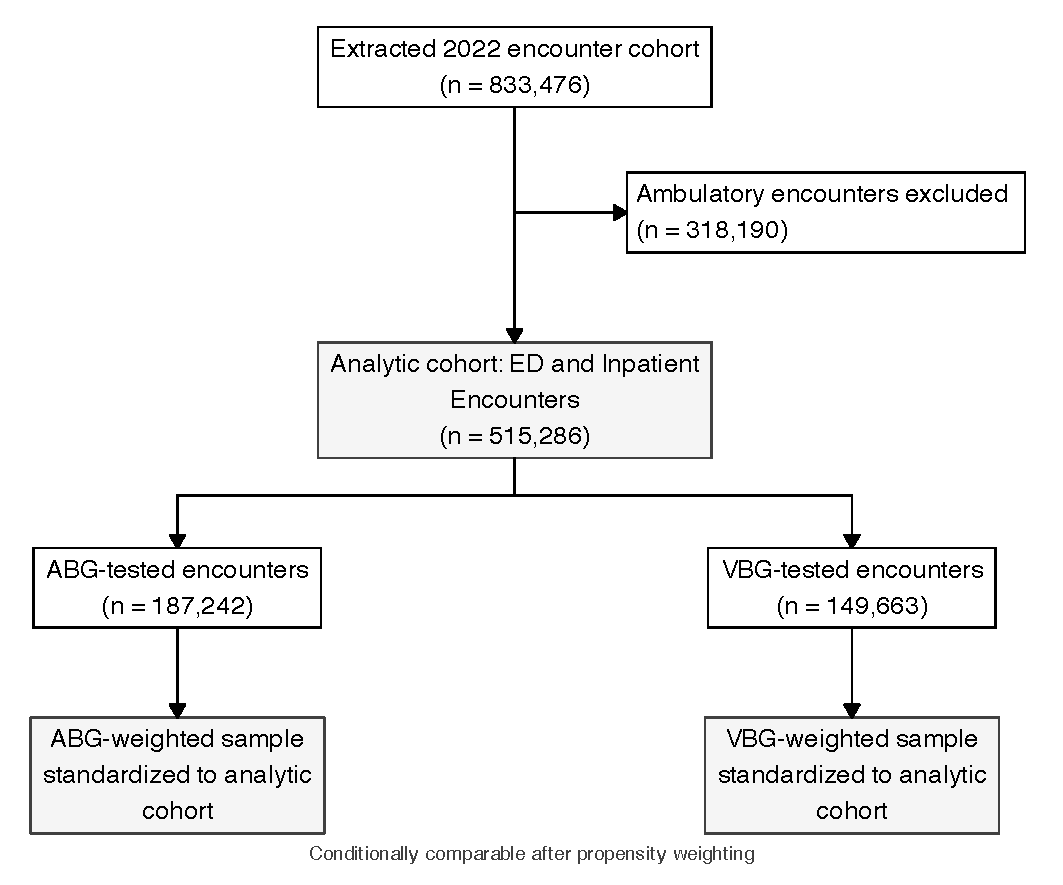
\includegraphics[width=0.88\linewidth,height=0.82\textheight,keepaspectratio]{Results/figs/figure_1_cohort_assembly_target_population_ipsw.pdf}

\end{minipage}
\end{center}

\clearpage
\begin{center}
\begin{minipage}{\linewidth}
\centering
\small Figure 2. Primary MI-logistic IPSW-weighted spline associations of pCO2 with clinical outcomes by ABG and VBG\par
\vspace{0.5em}
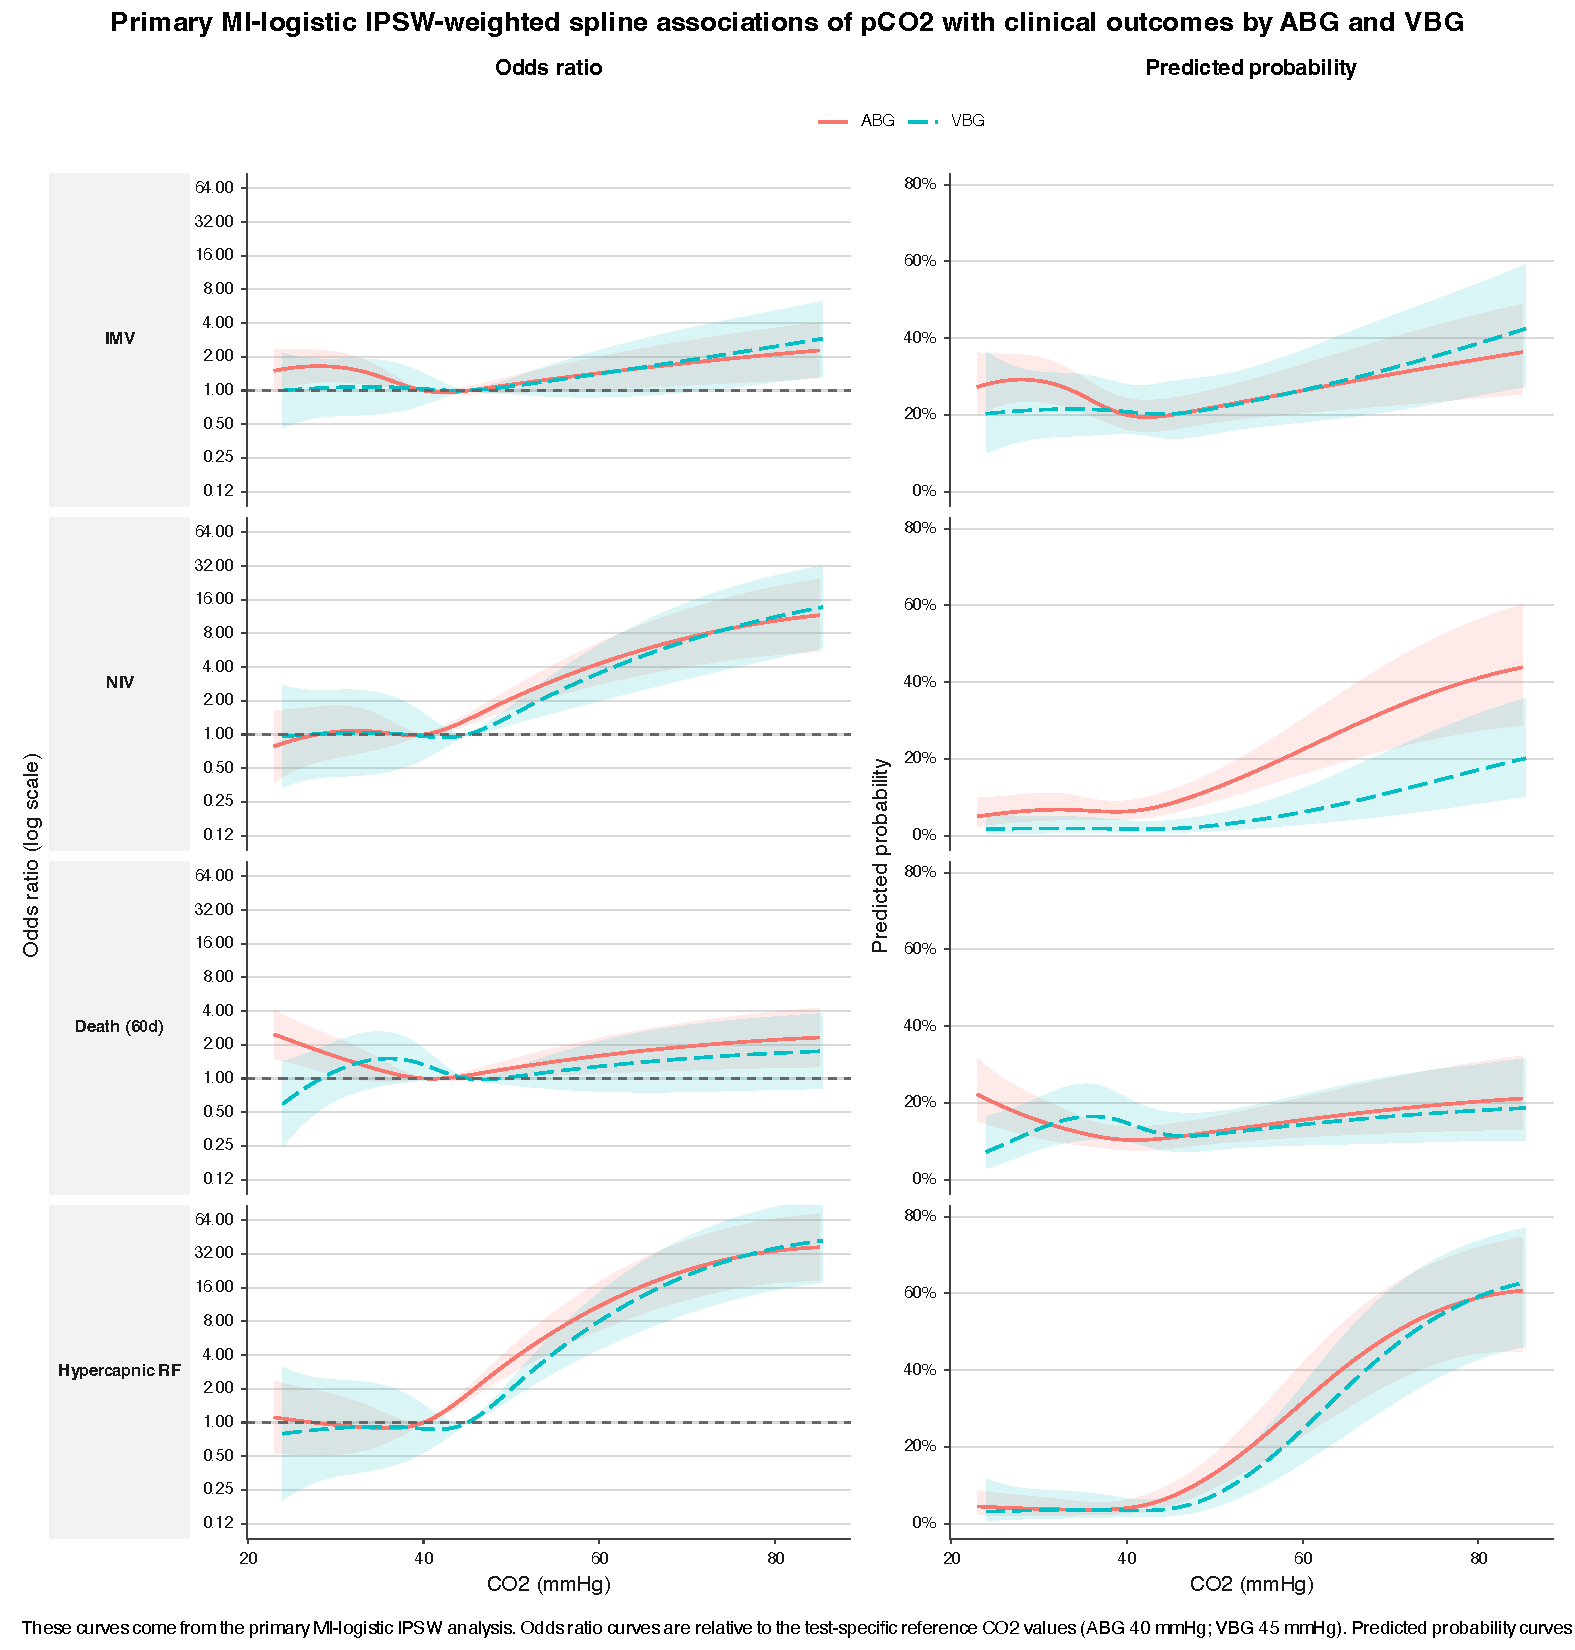
\includegraphics[width=0.88\linewidth,height=0.82\textheight,keepaspectratio]{Results/figs/figure_2_primary_weighted_spline_associations_abg_vbg.pdf}
\par\vspace{0.5em}\noindent\footnotesize Note: These curves come from the primary MI-logistic IPSW analysis. Odds ratio curves are relative to the test-specific reference CO2 values (ABG 40 mmHg; VBG 45 mmHg). Predicted probability curves are marginally standardized to the common eligible source-population covariate distribution.\normalsize
\end{minipage}
\end{center}

\clearpage

\begin{landscape}

\begin{center}\textbf{Table 1. Baseline characteristics of the analytic cohort overall and by receipt of arterial and venous blood gas testing}\end{center}

\begin{table}[!h]
\centering\begingroup\fontsize{6}{8}\selectfont

\resizebox{\ifdim\width>\linewidth\linewidth\else\width\fi}{!}{
\begin{tabular}{llllll}
\toprule
Characteristic & Everyone & Did not get ABG & Did get ABG & Did not get VBG & Did get VBG\\
\midrule
Age & 59.5 ± 17.6 & 58.4 ± 17.7 & 61.3 ± 17.2 & 59.6 ± 17.6 & 59.0 ± 17.7\\
BMI & 31.3 ± 8.5 & 32.6 ± 8.9 & 28.8 ± 7.0 & 31.9 ± 8.6 & 28.9 ± 7.5\\
Sex &  &  &  &  & \\
Female & 2,591 (50\%) & 1,737 (53\%) & 854 (45\%) & 1,921 (52\%) & 670 (46\%)\\
Male & 2,584 (50\%) & 1,527 (47\%) & 1,057 (55\%) & 1,809 (48\%) & 775 (54\%)\\
\addlinespace
Race/Ethnicity &  &  &  &  & \\
White & 3,280 (63\%) & 2,009 (62\%) & 1,271 (67\%) & 2,513 (67\%) & 767 (53\%)\\
Black or African American & 884 (17\%) & 601 (18\%) & 283 (15\%) & 616 (17\%) & 268 (19\%)\\
Hispanic & 334 (6.5\%) & 250 (7.7\%) & 84 (4.4\%) & 221 (5.9\%) & 113 (7.8\%)\\
Asian & 83 (1.6\%) & 46 (1.4\%) & 37 (1.9\%) & 54 (1.4\%) & 29 (2.0\%)\\
\addlinespace
American Indian & 36 (0.7\%) & 11 (0.3\%) & 25 (1.3\%) & 13 (0.3\%) & 23 (1.6\%)\\
Pacific Islander & 10 (0.2\%) & 8 (0.2\%) & 2 (0.1\%) & 8 (0.2\%) & 2 (0.1\%)\\
Unknown & 548 (11\%) & 339 (10\%) & 209 (11\%) & 305 (8.2\%) & 243 (17\%)\\
Location &  &  &  &  & \\
South & 2,431 (47\%) & 1,374 (42\%) & 1,057 (55\%) & 1,987 (53\%) & 444 (31\%)\\
\addlinespace
Northeast & 1,300 (25\%) & 921 (28\%) & 379 (20\%) & 703 (19\%) & 597 (41\%)\\
Midwest & 406 (7.8\%) & 246 (7.5\%) & 160 (8.4\%) & 264 (7.1\%) & 142 (9.8\%)\\
West & 1,038 (20\%) & 723 (22\%) & 315 (16\%) & 776 (21\%) & 262 (18\%)\\
OSA & 879 (17\%) & 576 (18\%) & 303 (16\%) & 648 (17\%) & 231 (16\%)\\
Asthma & 684 (13\%) & 464 (14\%) & 220 (12\%) & 513 (14\%) & 171 (12\%)\\
\addlinespace
COPD & 1,013 (20\%) & 579 (18\%) & 434 (23\%) & 731 (20\%) & 282 (20\%)\\
CHF & 1,044 (20\%) & 587 (18\%) & 457 (24\%) & 741 (20\%) & 303 (21\%)\\
NMD & 233 (4.5\%) & 130 (4.0\%) & 103 (5.4\%) & 175 (4.7\%) & 58 (4.0\%)\\
PHTN & 434 (8.4\%) & 239 (7.3\%) & 195 (10\%) & 295 (7.9\%) & 139 (9.6\%)\\
CKD & 904 (17\%) & 519 (16\%) & 385 (20\%) & 628 (17\%) & 276 (19\%)\\
\addlinespace
Diabetes & 1,513 (29\%) & 954 (29\%) & 559 (29\%) & 1,034 (28\%) & 479 (33\%)\\
Encounter Type &  &  &  &  & \\
Emergency & 1,710 (33\%) & 1,427 (44\%) & 283 (15\%) & 1,247 (33\%) & 463 (32\%)\\
Inpatient & 3,465 (67\%) & 1,837 (56\%) & 1,628 (85\%) & 2,483 (67\%) & 982 (68\%)\\
\bottomrule
\end{tabular}}
\endgroup{}
\end{table}

\end{landscape}

\clearpage

\begin{landscape}

\begin{center}\textbf{Table 2. MI-pooled, MI-logistic IPSW-weighted 3-level categorical results for ABG and VBG}\end{center}

\medskip\noindent\textbf{Panel A. Odds ratios}\par

\begin{table}[!h]
\centering\begingroup\fontsize{7}{9}\selectfont

\resizebox{\ifdim\width>\linewidth\linewidth\else\width\fi}{!}{
\begin{tabular}{llrrll}
\toprule
Gas type & Outcome & Analysis N & Events & Low vs normal OR (95\% CI) & High vs normal OR (95\% CI)\\
\midrule
ABG & IMV & 1911 & 463 & 1.41 (1.05, 1.90) & 1.26 (0.93, 1.71)\\
VBG & IMV & 1445 & 208 & 1.24 (0.77, 2.00) & 1.63 (1.02, 2.60)\\
ABG & NIV & 1911 & 183 & 1.04 (0.63, 1.72) & 3.05 (1.99, 4.68)\\
VBG & NIV & 1445 & 100 & 0.76 (0.38, 1.52) & 2.69 (1.47, 4.90)\\
ABG & Death (60d) & 1911 & 322 & 1.55 (1.07, 2.25) & 1.50 (1.06, 2.14)\\
\addlinespace
VBG & Death (60d) & 1445 & 200 & 1.10 (0.68, 1.79) & 1.10 (0.70, 1.74)\\
ABG & Hypercapnic RF & 1911 & 206 & 1.26 (0.70, 2.26) & 9.21 (5.73, 14.81)\\
VBG & Hypercapnic RF & 1445 & 133 & 0.68 (0.30, 1.54) & 6.28 (3.50, 11.25)\\
\bottomrule
\end{tabular}}
\endgroup{}
\end{table}

\medskip\noindent\textbf{Panel B. Predicted probabilities}\par

\begin{table}[!h]
\centering\begingroup\fontsize{7}{9}\selectfont

\resizebox{\ifdim\width>\linewidth\linewidth\else\width\fi}{!}{
\begin{tabular}{lllll}
\toprule
Gas type & Outcome & Normal probability (95\% CI) & Low probability (95\% CI) & High probability (95\% CI)\\
\midrule
ABG & IMV & 0.18 (0.15, 0.21) & 0.23 (0.19, 0.27) & 0.21 (0.18, 0.25)\\
VBG & IMV & 0.11 (0.09, 0.15) & 0.13 (0.10, 0.18) & 0.17 (0.13, 0.21)\\
ABG & NIV & 0.06 (0.04, 0.08) & 0.06 (0.04, 0.09) & 0.15 (0.12, 0.19)\\
VBG & NIV & 0.06 (0.04, 0.09) & 0.05 (0.03, 0.08) & 0.14 (0.10, 0.19)\\
ABG & Death (60d) & 0.11 (0.09, 0.14) & 0.16 (0.13, 0.20) & 0.16 (0.13, 0.19)\\
\addlinespace
VBG & Death (60d) & 0.11 (0.08, 0.14) & 0.12 (0.09, 0.15) & 0.12 (0.09, 0.15)\\
ABG & Hypercapnic RF & 0.03 (0.02, 0.05) & 0.04 (0.03, 0.06) & 0.23 (0.19, 0.28)\\
VBG & Hypercapnic RF & 0.05 (0.03, 0.07) & 0.03 (0.02, 0.06) & 0.22 (0.17, 0.27)\\
\bottomrule
\end{tabular}}
\endgroup{}
\end{table}

\end{landscape}

\clearpage

\begin{landscape}

\begin{center}\textbf{Table S1. Inclusion criteria into the enriched sample}\end{center}

\begin{table}[!h]
\centering\begingroup\fontsize{6}{8}\selectfont

\resizebox{\ifdim\width>\linewidth\linewidth\else\width\fi}{!}{
\begin{tabular}{lllllll}
\toprule
Phenotype input & Code system & Source code/value or extract field & Analysis field(s) & Role & Source code status & Notes\\
\midrule
Arterial blood gas measurement & LOINC-derived laboratory field & value\_highest\_20198 & value\_highest\_20198; paco2; has\_abg & Source-cohort enrichment; ABG exposure definition & available extract concept identifier; upstream LOINC code list not available in analysis extract & Imported ABG-related concept field used in the arterial CO2 derivation.\\
Arterial blood gas measurement & LOINC-derived laboratory field & value\_highest\_115576 & value\_highest\_115576; abg\_ph; has\_abg & Source-cohort enrichment; ABG exposure definition & available extract concept identifier; upstream LOINC code list not available in analysis extract & Imported ABG-related concept field retained with the arterial gas measurement set.\\
Arterial blood gas measurement & LOINC-derived laboratory field & value\_highest\_327718 & value\_highest\_327718; abg\_hco3; abg\_o2sat; has\_abg & Source-cohort enrichment; ABG exposure definition & available extract concept identifier; upstream LOINC code list not available in analysis extract & Imported ABG-related concept field retained with arterial bicarbonate/O2-saturation fields.\\
Arterial blood gas procedure & LOINC/procedure-derived flag & meas\_arterial\_gas\_proc; meas\_art\_gas\_proc\_first\_date & meas\_arterial\_gas\_proc; meas\_art\_gas\_proc\_first\_date; has\_abg & Source-cohort enrichment; ABG exposure definition; timing diagnostics & collapsed derived procedure flag; upstream source code list not available in analysis extract & Procedure-date field is an encounter-day offset when present.\\
Venous blood gas measurement & LOINC-derived laboratory field & vbg\_co2; vbg\_ph; vbg\_hco3; vbg\_o2sat & vbg\_co2; vbg\_ph; vbg\_hco3; vbg\_o2sat; has\_vbg & Source-cohort enrichment; VBG exposure definition & collapsed derived measurement fields; upstream LOINC code list not available in analysis extract & The de-identified analysis extract stores VBG measurement variables rather than row-level LOINC code rows.\\
\addlinespace
Venous blood gas procedure & LOINC/procedure-derived flag & meas\_venous\_o2\_proc; meas\_venous\_o2\_proc\_first\_date & meas\_venous\_o2\_proc; meas\_venous\_o2\_proc\_first\_date; has\_vbg & Source-cohort enrichment; VBG exposure definition; timing diagnostics & collapsed derived procedure flag; upstream source code list not available in analysis extract & Procedure-date field is an encounter-day offset when present.\\
Hypercapnic respiratory failure and related respiratory diagnoses & ICD-10-CM-derived diagnosis flags & hypercap\_resp\_failure; resp\_acid\_dx; other\_resp\_failure; resp\_abnormality; resp\_dep\_compl; RESPFAIL\_rfs & hypercap\_resp\_failure; resp\_acid\_dx; other\_resp\_failure; resp\_abnormality; resp\_dep\_compl; RESPFAIL\_rfs & Source-cohort enrichment; hypercapnic respiratory failure outcome definition & collapsed derived diagnosis flags; upstream ICD-10-CM code list not available in analysis extract & These fields identify respiratory-failure phenotypes after upstream code grouping.\\
Severe obesity, OHS, and sleep-hypoventilation criteria & ICD-10-CM-derived flags and measured BMI fields & ohs\_code; sleep\_hypovent\_dx; other\_sleep\_hypovent\_dx; curr\_bmi; working\_bmi; bmi; ats\_ohs\_flag; pos\_ohs\_flag; OBESITY\_rfs & ohs\_code; sleep\_hypovent\_dx; other\_sleep\_hypovent\_dx; curr\_bmi; working\_bmi; bmi; ats\_ohs\_flag; pos\_ohs\_flag; OBESITY\_rfs & Source-cohort enrichment; covariate definition & mixed measured fields and collapsed derived diagnosis flags; upstream ICD-10-CM code list not available in analysis extract & BMI is retained as a baseline covariate; OHS and obesity flags support enriched-cohort construction.\\
Non-invasive ventilation procedure & CPT/PCS/procedure-derived flag & niv\_proc; niv\_proc\_first\_date & niv\_proc; niv\_proc\_first\_date; VENTSUPPORT\_rfs & Source-cohort enrichment; NIV outcome definition; timing diagnostics & collapsed derived procedure flag; upstream CPT/PCS/procedure code list not available in analysis extract & The date field is an encounter-day offset and is used only for diagnostic timing sensitivity.\\
Invasive mechanical ventilation procedure & CPT/PCS/procedure-derived flag & imv\_proc; imv\_proc\_first\_date & imv\_proc; imv\_proc\_first\_date; VENTSUPPORT\_rfs & Source-cohort enrichment; IMV outcome definition; timing diagnostics & collapsed derived procedure flag; upstream CPT/PCS/procedure code list not available in analysis extract & The date field is an encounter-day offset and is used only for diagnostic timing sensitivity.\\
\addlinespace
Any ventilatory support procedure & CPT/PCS/procedure-derived flag & vent\_proc; vent\_proc\_first\_date; VENTSUPPORT\_rfs & vent\_proc; vent\_proc\_first\_date; VENTSUPPORT\_rfs & Source-cohort enrichment; ventilatory-support phenotype definition & collapsed derived procedure flag; upstream CPT/PCS/procedure code list not available in analysis extract & Composite ventilatory-support fields combine NIV and IMV-related upstream procedure groupings.\\
\bottomrule
\end{tabular}}
\endgroup{}
\end{table}

\end{landscape}

\clearpage
\begin{center}
\begin{minipage}{\linewidth}
\centering
\small Figure S1. Covariate balance after MI logistic inverse-probability weighting for ABG and VBG test-ordering models\par
\vspace{0.5em}
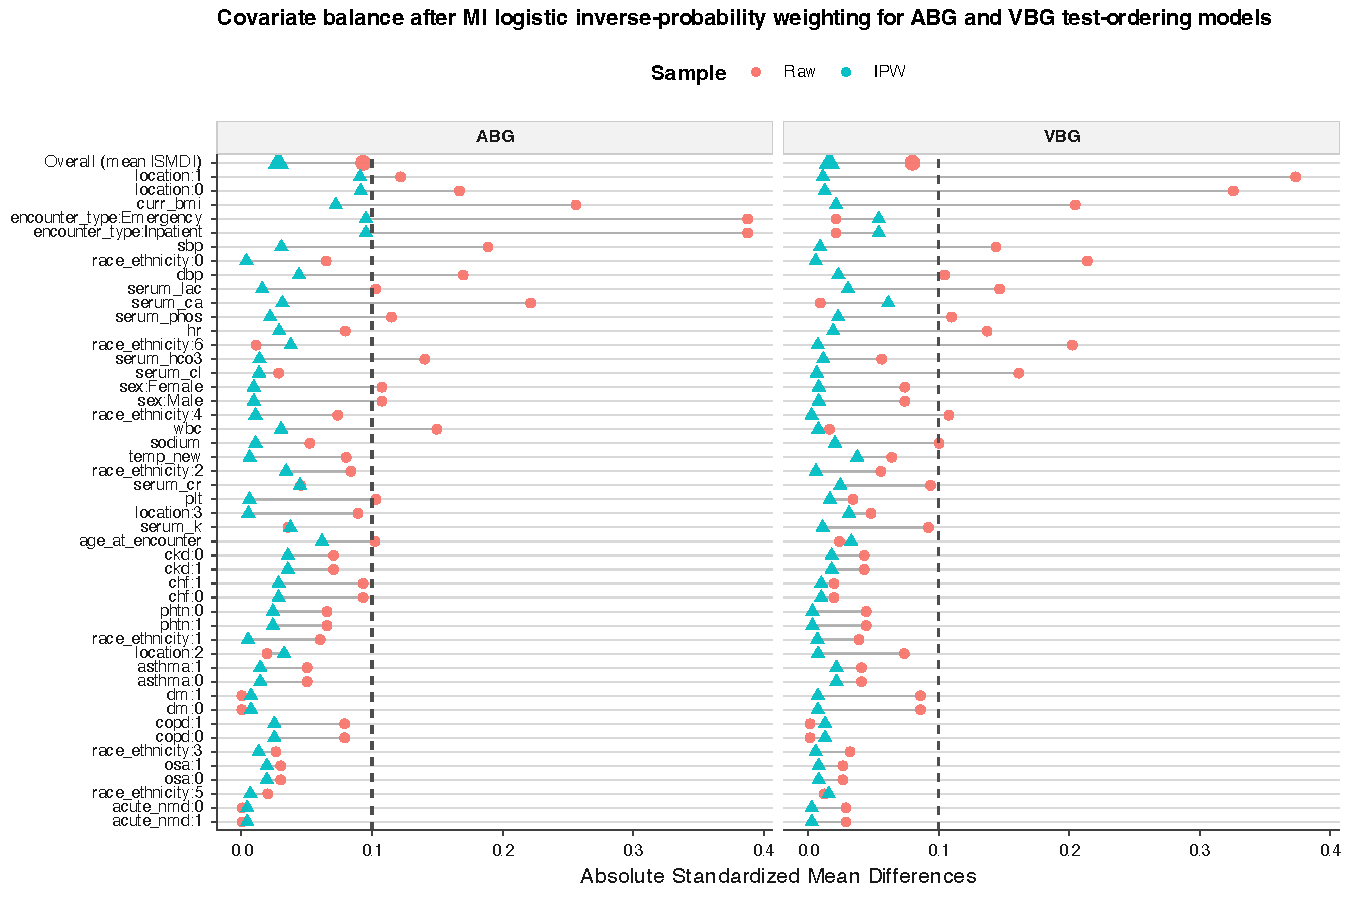
\includegraphics[width=0.88\linewidth,height=0.82\textheight,keepaspectratio]{Results/figs/figure_s1_covariate_balance_mi_logistic_ipsw.pdf}

\end{minipage}
\end{center}

\clearpage
\begin{center}
\begin{minipage}{\linewidth}
\centering
\small Figure S2. Propensity-score overlap for MI logistic ABG and VBG test-ordering models\par
\vspace{0.5em}
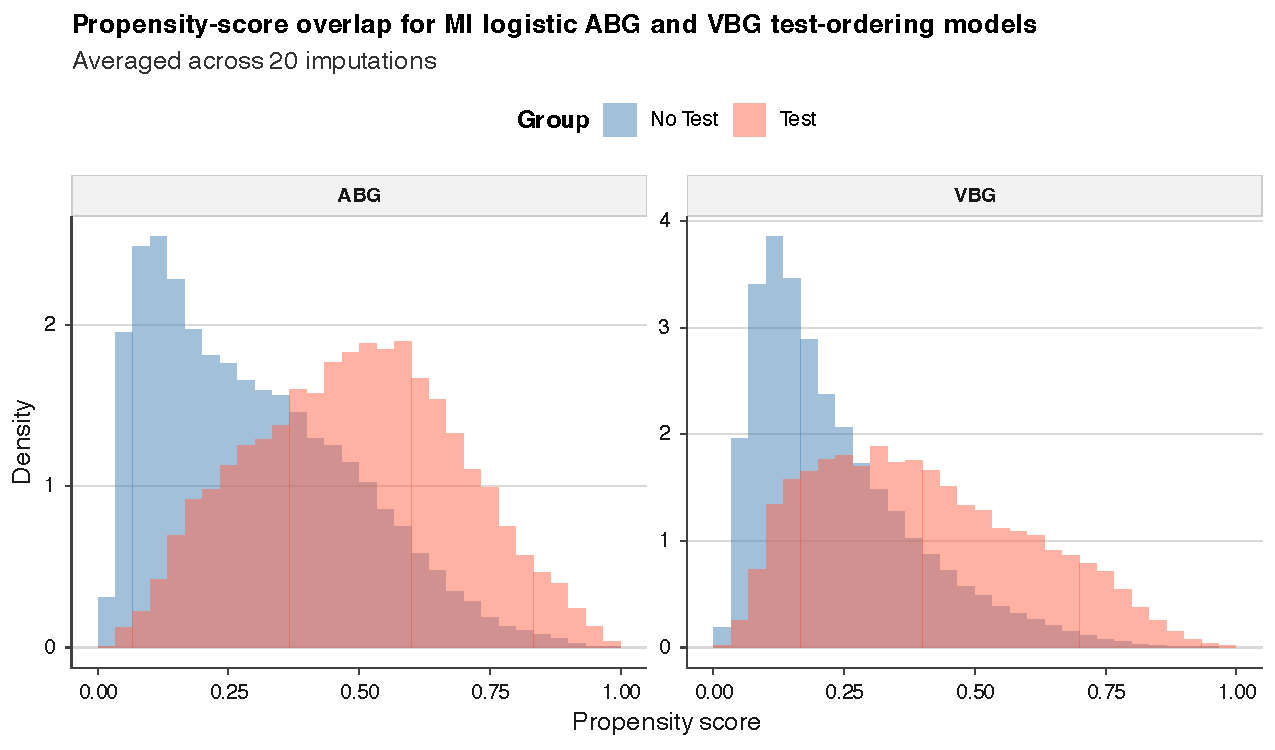
\includegraphics[width=0.88\linewidth,height=0.82\textheight,keepaspectratio]{Results/figs/figure_s2_propensity_score_overlap_mi_logistic.pdf}

\end{minipage}
\end{center}

\clearpage
\begin{center}
\begin{minipage}{\linewidth}
\centering
\small Figure S3. SHAP-style contribution summaries for MI logistic ABG and VBG test-ordering models\par
\vspace{0.5em}
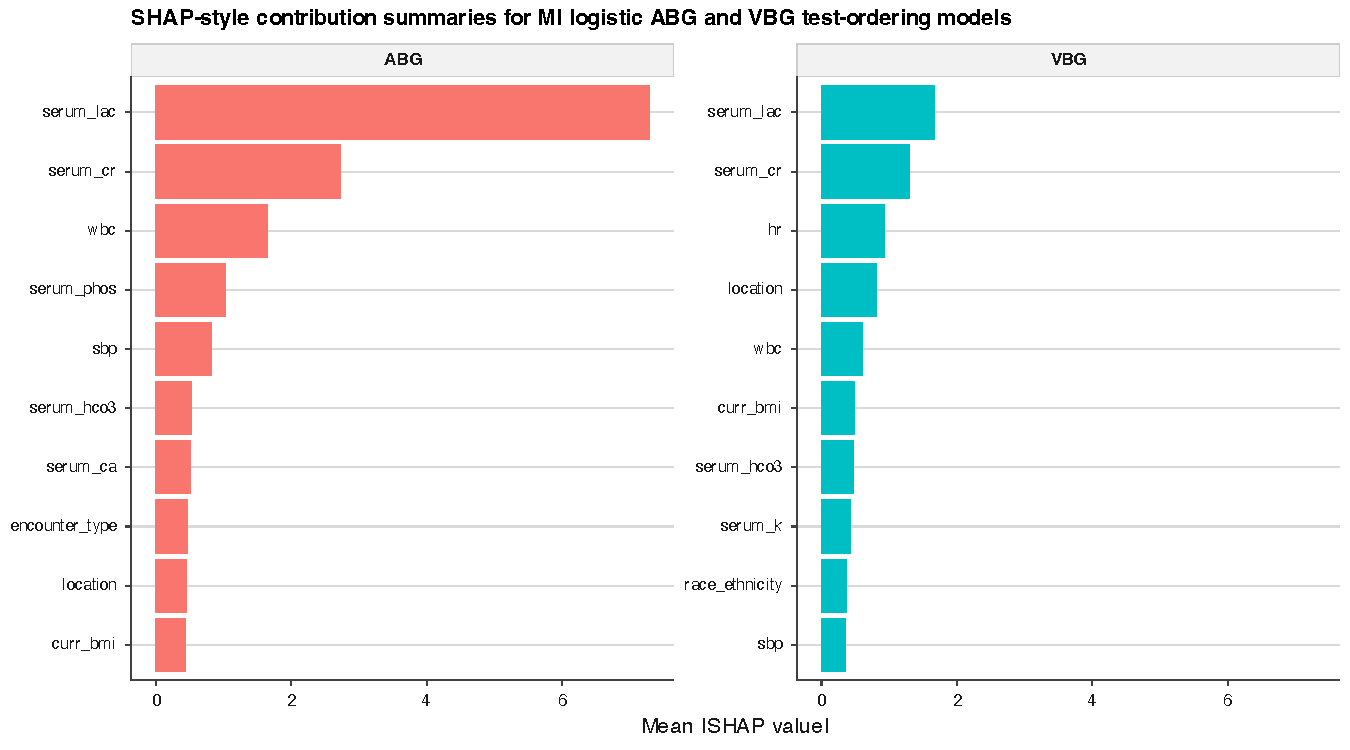
\includegraphics[width=0.88\linewidth,height=0.82\textheight,keepaspectratio]{Results/figs/figure_s3_shap_style_contributions_mi_logistic.pdf}

\end{minipage}
\end{center}

\clearpage
\begin{center}
\begin{minipage}{\linewidth}
\centering
\small Figure S4. MI-logistic IPSW-weighted categorical associations of pCO2 category with clinical outcomes by ABG and VBG\par
\vspace{0.5em}
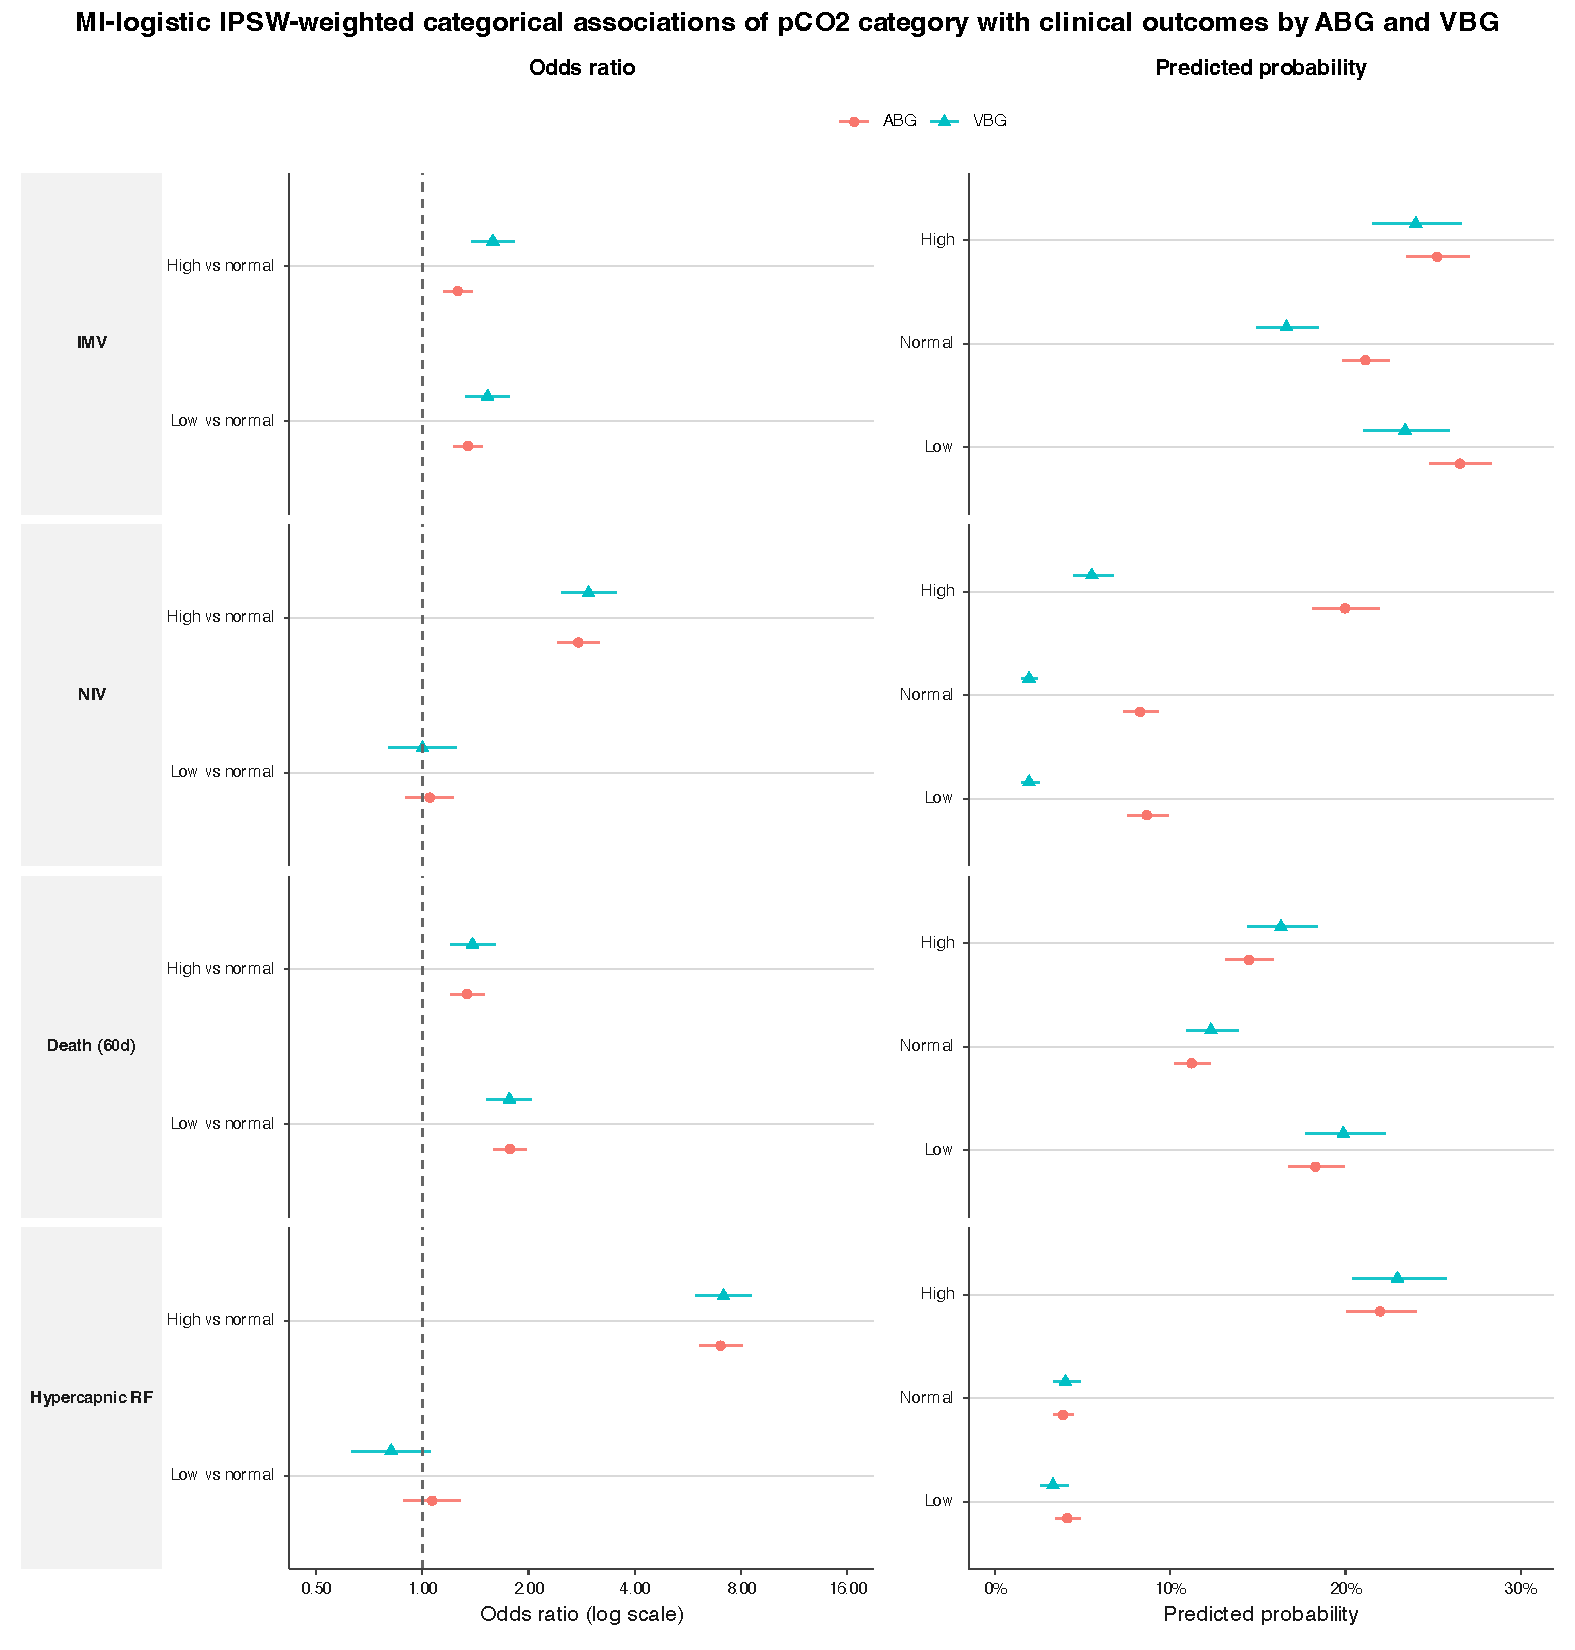
\includegraphics[width=0.88\linewidth,height=0.82\textheight,keepaspectratio]{Results/figs/figure_s4_weighted_categorical_associations_abg_vbg.pdf}
\par\vspace{0.5em}\noindent\footnotesize Note: MI-pooled, MI-logistic IPSW-adjusted categorical odds ratios use the normal CO2 category as the reference. Predicted probabilities are pooled on the link scale and marginally standardized to the common eligible source-population covariate distribution.\normalsize
\end{minipage}
\end{center}

\clearpage
\begin{center}
\begin{minipage}{\linewidth}
\centering
\small Figure S5. Unweighted covariate-adjusted spline associations of pCO2 with clinical outcomes by ABG and VBG\par
\vspace{0.5em}
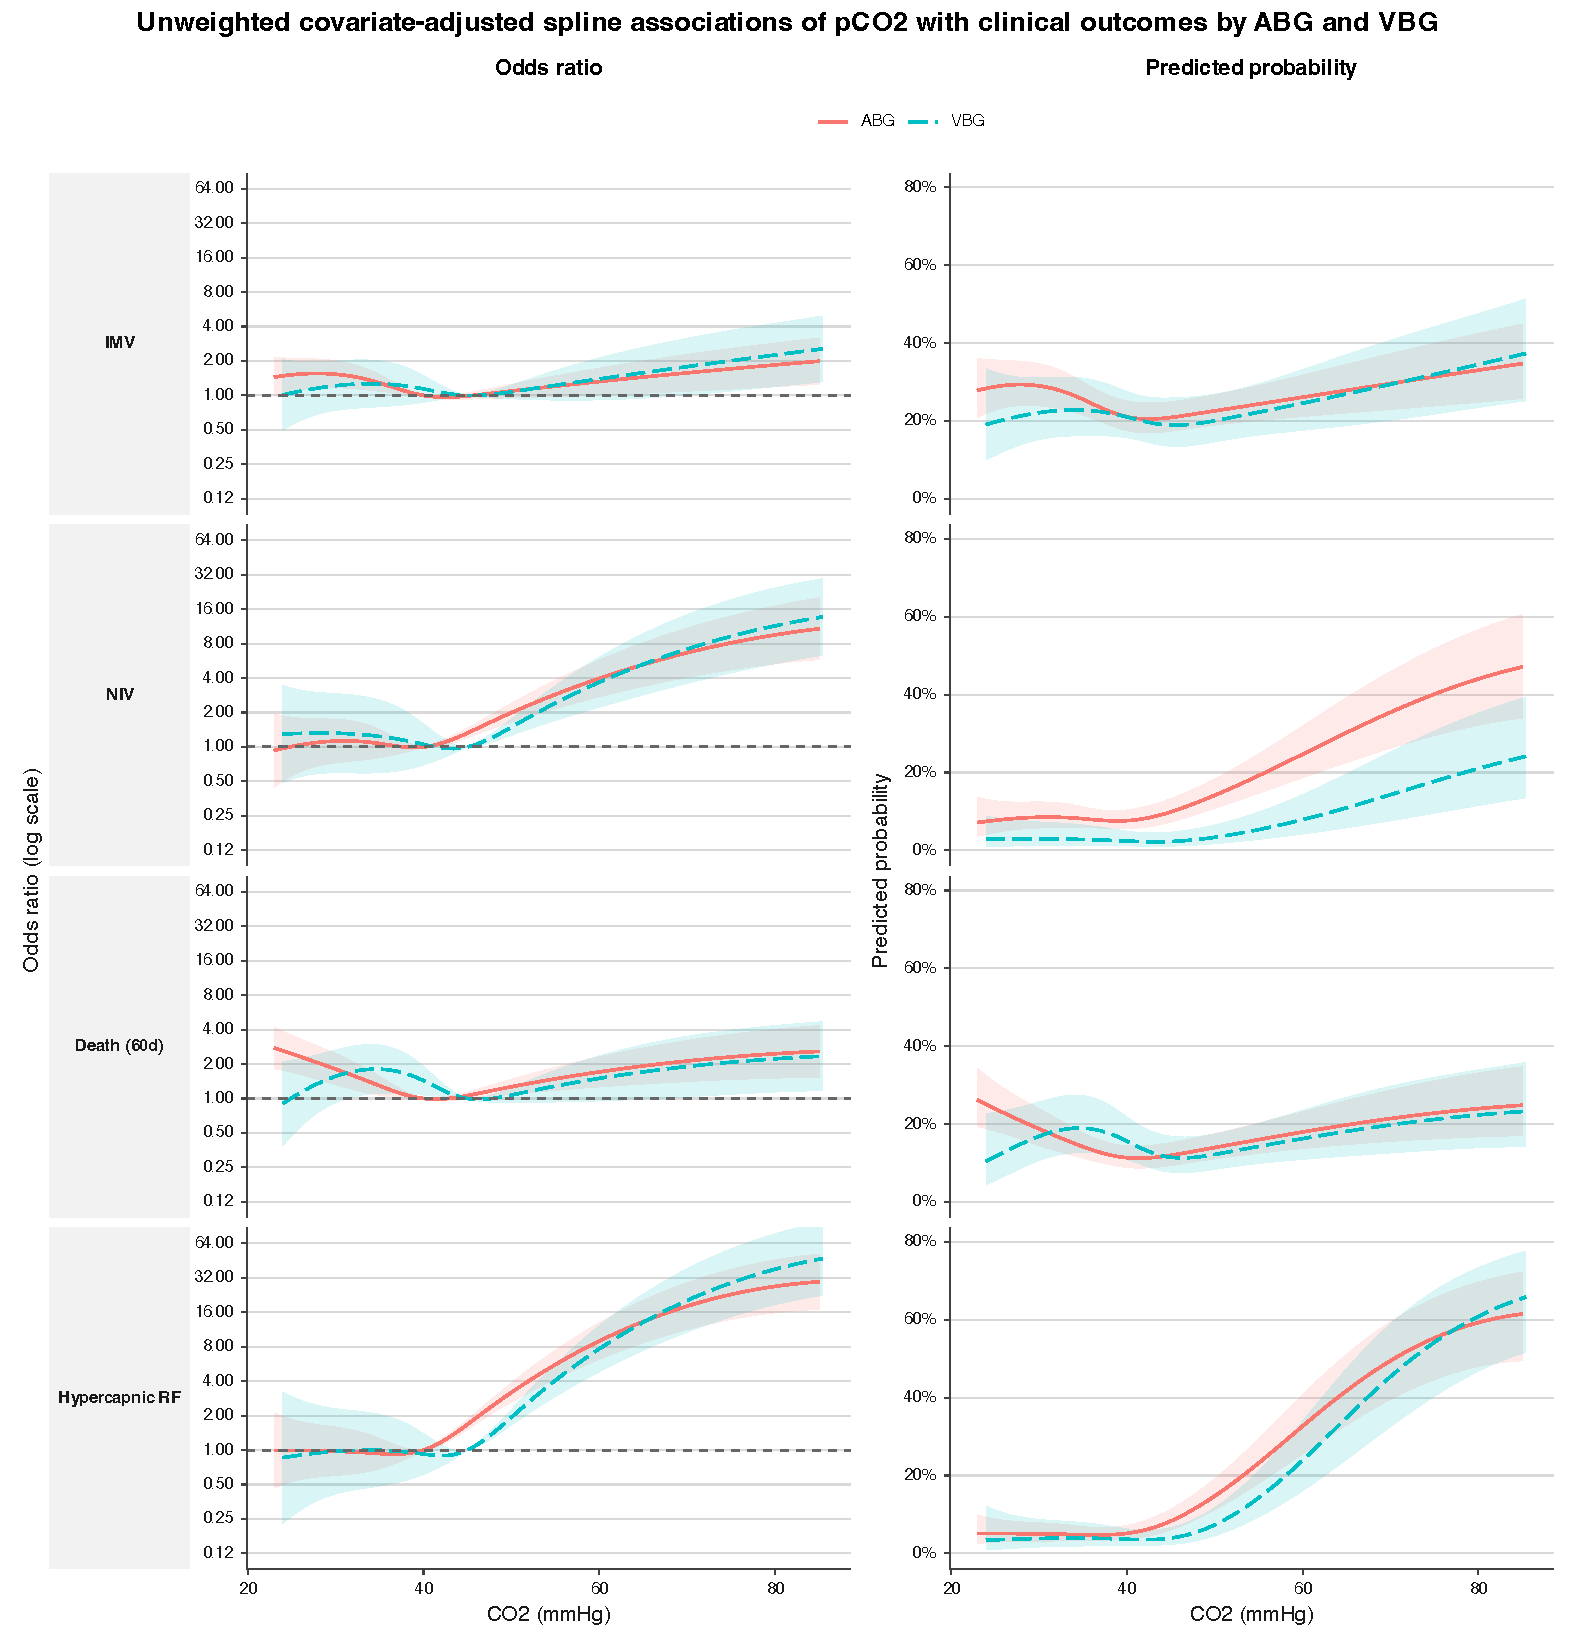
\includegraphics[width=0.88\linewidth,height=0.82\textheight,keepaspectratio]{Results/figs/figure_s5_unweighted_adjusted_spline_abg_vbg.pdf}
\par\vspace{0.5em}\noindent\footnotesize Note: Odds ratio curves are relative to the test-specific reference CO2 values (ABG 40 mmHg; VBG 45 mmHg). Predicted probability curves are conditional on the reference covariate profile X\_ref within each test-specific cohort.\normalsize
\end{minipage}
\end{center}

\clearpage

\begin{landscape}

\begin{center}\textbf{Table S2. Crude associations of pCO2 category with clinical outcomes by ABG and VBG}\end{center}

\begin{table}[!h]
\centering\begingroup\fontsize{6}{8}\selectfont

\resizebox{\ifdim\width>\linewidth\linewidth\else\width\fi}{!}{
\begin{tabular}{llll}
\toprule
Gas type & Outcome & Contrast & OR (95\% CI)\\
\midrule
ABG & IMV & Low vs normal & 1.44 (1.12, 1.86)\\
ABG & IMV & High vs normal & 1.28 (0.99, 1.65)\\
VBG & IMV & Low vs normal & 1.48 (1.03, 2.13)\\
VBG & IMV & High vs normal & 1.80 (1.27, 2.57)\\
ABG & NIV & Low vs normal & 1.00 (0.65, 1.52)\\
\addlinespace
ABG & NIV & High vs normal & 2.26 (1.60, 3.21)\\
VBG & NIV & Low vs normal & 1.21 (0.69, 2.09)\\
VBG & NIV & High vs normal & 2.61 (1.63, 4.23)\\
ABG & Death (60d) & Low vs normal & 1.60 (1.19, 2.15)\\
ABG & Death (60d) & High vs normal & 1.55 (1.16, 2.08)\\
\addlinespace
VBG & Death (60d) & Low vs normal & 1.71 (1.19, 2.45)\\
VBG & Death (60d) & High vs normal & 1.58 (1.10, 2.29)\\
ABG & Hypercapnic RF & Low vs normal & 1.36 (0.81, 2.28)\\
ABG & Hypercapnic RF & High vs normal & 8.29 (5.65, 12.50)\\
VBG & Hypercapnic RF & Low vs normal & 0.99 (0.51, 1.85)\\
\addlinespace
VBG & Hypercapnic RF & High vs normal & 7.13 (4.58, 11.46)\\
\bottomrule
\end{tabular}}
\endgroup{}
\end{table}

\end{landscape}

\clearpage

\begin{landscape}

\begin{center}\textbf{Table S3. GBM IPSW-weighted associations of pCO2 category with clinical outcomes by ABG and VBG}\end{center}

\begin{table}[!h]
\centering\begingroup\fontsize{6}{8}\selectfont

\resizebox{\ifdim\width>\linewidth\linewidth\else\width\fi}{!}{
\begin{tabular}{llll}
\toprule
Gas type & Outcome & Contrast & OR (95\% CI)\\
\midrule
ABG & IMV & Low vs normal & 1.40 (1.06, 1.86)\\
ABG & IMV & High vs normal & 1.14 (0.85, 1.52)\\
VBG & IMV & Low vs normal & 1.34 (0.89, 2.03)\\
VBG & IMV & High vs normal & 1.58 (1.06, 2.37)\\
ABG & NIV & Low vs normal & 1.04 (0.65, 1.69)\\
\addlinespace
ABG & NIV & High vs normal & 2.82 (1.90, 4.17)\\
VBG & NIV & Low vs normal & 0.88 (0.47, 1.67)\\
VBG & NIV & High vs normal & 2.77 (1.62, 4.75)\\
ABG & Death (60d) & Low vs normal & 1.52 (1.08, 2.16)\\
ABG & Death (60d) & High vs normal & 1.46 (1.05, 2.02)\\
\addlinespace
VBG & Death (60d) & Low vs normal & 1.38 (0.91, 2.10)\\
VBG & Death (60d) & High vs normal & 1.31 (0.87, 1.98)\\
ABG & Hypercapnic RF & Low vs normal & 1.54 (0.84, 2.82)\\
ABG & Hypercapnic RF & High vs normal & 9.39 (5.99, 14.73)\\
VBG & Hypercapnic RF & Low vs normal & 0.76 (0.37, 1.56)\\
\addlinespace
VBG & Hypercapnic RF & High vs normal & 7.58 (4.54, 12.67)\\
\bottomrule
\end{tabular}}
\endgroup{}
\end{table}

\end{landscape}

\clearpage
\begin{center}
\begin{minipage}{\linewidth}
\centering
\small Figure S6. Covariate balance after gradient-boosted propensity weighting for ABG and VBG test-ordering models\par
\vspace{0.5em}
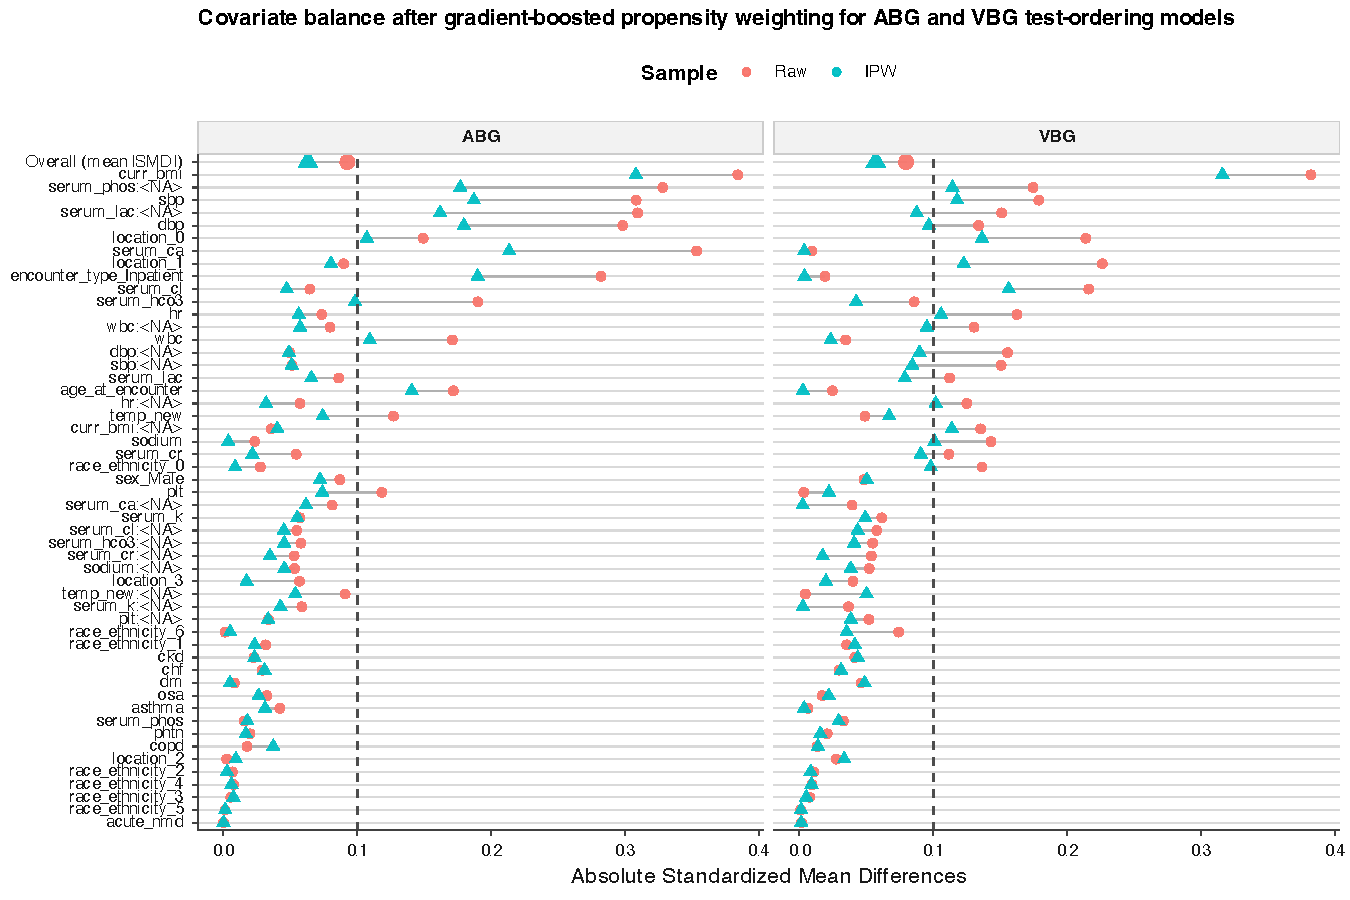
\includegraphics[width=0.88\linewidth,height=0.82\textheight,keepaspectratio]{Results/figs/figure_s6_covariate_balance_gbm_weighting.pdf}

\end{minipage}
\end{center}

\clearpage
\begin{center}
\begin{minipage}{\linewidth}
\centering
\small Figure S7. Propensity-score overlap for gradient-boosted ABG and VBG test-ordering models\par
\vspace{0.5em}
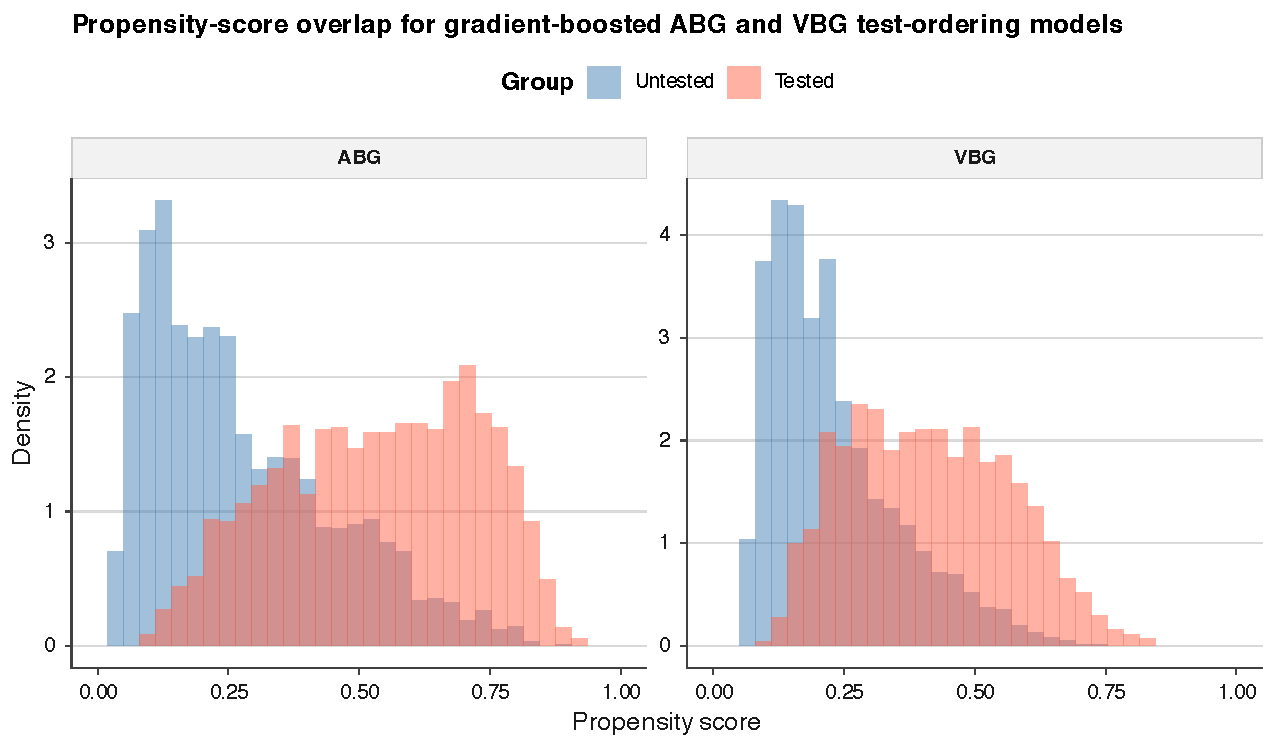
\includegraphics[width=0.88\linewidth,height=0.82\textheight,keepaspectratio]{Results/figs/figure_s7_propensity_score_overlap_gbm.pdf}

\end{minipage}
\end{center}

\clearpage
\begin{center}
\begin{minipage}{\linewidth}
\centering
\small Figure S8. SHAP-style contribution summaries for gradient-boosted ABG and VBG test-ordering models\par
\vspace{0.5em}
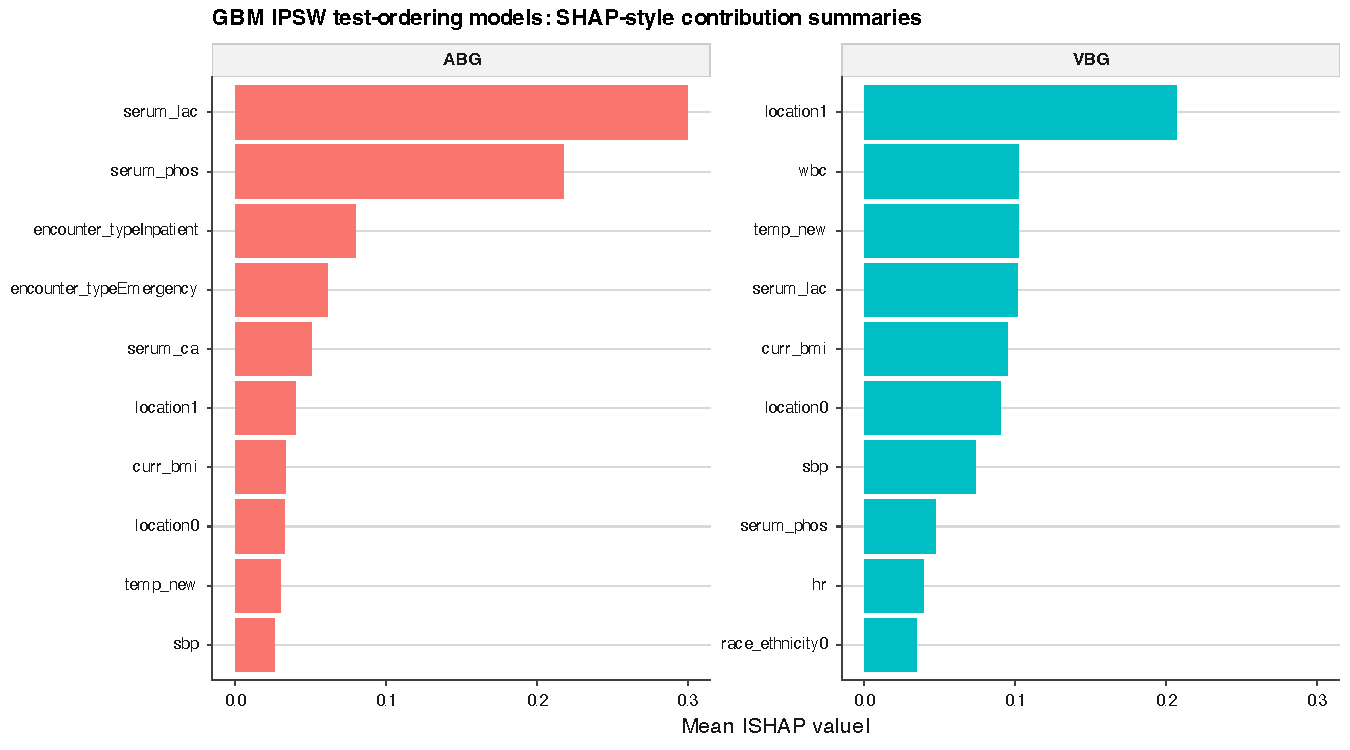
\includegraphics[width=0.88\linewidth,height=0.82\textheight,keepaspectratio]{Results/figs/figure_s8_shap_style_contributions_gbm.pdf}

\end{minipage}
\end{center}

\clearpage

\begin{landscape}

\begin{center}\textbf{Table S4. Missingness of baseline covariates used in the primary analysis}\end{center}

\begin{table}[!h]
\centering\begingroup\fontsize{7}{9}\selectfont

\resizebox{\ifdim\width>\linewidth\linewidth\else\width\fi}{!}{
\begin{tabular}{lllllll}
\toprule
Variable & Analysis role & \% missing & Included in MI model & Imputed if missing & Observed complete & Notes\\
\midrule
Age & direct adjustment; PS model & 0.0\% & Yes & No & Yes & Complete in this render; used as MI predictor or model variable.\\
Sex & direct adjustment; PS model & 0.0\% & Yes & No & Yes & Complete in this render; used as MI predictor or model variable.\\
Race/ethnicity & direct adjustment; PS model & 0.0\% & Yes & No & Yes & Complete in this render; used as MI predictor or model variable.\\
BMI & PS model & 56.7\% & Yes & Yes & No & Eligible for MICE method: pmm.\\
COPD & PS model & 0.0\% & Yes & No & Yes & Complete in this render; used as MI predictor or model variable.\\
\addlinespace
Asthma & PS model & 0.0\% & Yes & No & Yes & Complete in this render; used as MI predictor or model variable.\\
OSA & PS model & 0.0\% & Yes & No & Yes & Complete in this render; used as MI predictor or model variable.\\
CHF & PS model & 0.0\% & Yes & No & Yes & Complete in this render; used as MI predictor or model variable.\\
Neuromuscular disease & PS model & 0.0\% & Yes & No & Yes & Complete in this render; used as MI predictor or model variable.\\
Pulmonary hypertension & PS model & 0.0\% & Yes & No & Yes & Complete in this render; used as MI predictor or model variable.\\
\addlinespace
Chronic kidney disease & PS model & 0.0\% & Yes & No & Yes & Complete in this render; used as MI predictor or model variable.\\
Diabetes & PS model & 0.0\% & Yes & No & Yes & Complete in this render; used as MI predictor or model variable.\\
Location & direct adjustment; PS model & 0.0\% & Yes & No & Yes & Complete in this render; used as MI predictor or model variable.\\
Encounter type & direct adjustment; PS model & 0.0\% & Yes & No & Yes & Complete in this render; used as MI predictor or model variable.\\
Temperature & PS model & 48.3\% & Yes & Yes & No & Eligible for MICE method: pmm.\\
\addlinespace
Systolic blood pressure & PS model & 29.8\% & Yes & Yes & No & Eligible for MICE method: pmm.\\
Diastolic blood pressure & PS model & 30.1\% & Yes & Yes & No & Eligible for MICE method: pmm.\\
Heart rate & PS model & 36.5\% & Yes & Yes & No & Eligible for MICE method: pmm.\\
Sodium & PS model & 5.0\% & Yes & Yes & No & Eligible for MICE method: pmm.\\
Serum creatinine & PS model & 9.3\% & Yes & Yes & No & Eligible for MICE method: pmm.\\
\addlinespace
Serum bicarbonate & PS model & 5.4\% & Yes & Yes & No & Eligible for MICE method: pmm.\\
Serum chloride & PS model & 5.8\% & Yes & Yes & No & Eligible for MICE method: pmm.\\
Serum lactate & PS model & 60.4\% & Yes & Yes & No & Eligible for MICE method: pmm.\\
Serum potassium & PS model & 7.8\% & Yes & Yes & No & Eligible for MICE method: pmm.\\
White blood cell count & PS model & 17.3\% & Yes & Yes & No & Eligible for MICE method: pmm.\\
\addlinespace
Platelet count & PS model & 7.7\% & Yes & Yes & No & Eligible for MICE method: pmm.\\
Serum phosphate & PS model & 52.8\% & Yes & Yes & No & Eligible for MICE method: pmm.\\
Serum calcium & PS model & 10.0\% & Yes & Yes & No & Eligible for MICE method: pmm.\\
\bottomrule
\end{tabular}}
\endgroup{}
\end{table}

\end{landscape}

\clearpage

\begin{landscape}

\begin{center}\textbf{Table S5. Multiple-imputation diagnostic summary}\end{center}

\begin{table}[!h]
\centering\begingroup\fontsize{6}{8}\selectfont

\resizebox{\ifdim\width>\linewidth\linewidth\else\width\fi}{!}{
\begin{tabular}{llll}
\toprule
Domain & Metric & Value & Status\\
\midrule
Render scope & Current render & pilot (pilot\_frac=0.01) & warning\\
Render scope & Final manuscript target & full (m=80; maxit=20) & not applicable\\
Imputation run & Completed imputations & 20 & resolved\\
Imputation run & Iterations per imputation & 5 & resolved\\
Imputation run & Variables imputed & 16 & resolved\\
\addlinespace
Monte Carlo error & Maximum MC error / SE in diagnostic model & 0.177 & resolved\\
Chain diagnostics & Variables with available chain diagnostics & 16 & resolved\\
Chain diagnostics & Variables flagged for drift & 14 & warning\\
MICE logged events & Total logged events & 110 & warning\\
Captured warnings & Captured warning rows & 0 & resolved\\
\addlinespace
Outcome fit diagnostics & MI model fits audited & 692 & resolved\\
Outcome fit diagnostics & Fits with nonconvergence flags & 0 & resolved\\
Outcome fit diagnostics & Fits with explicit separation warnings & 0 & resolved\\
Outcome fit diagnostics & Fits with tail-only fitted-probability warnings & 540 & warning\\
\bottomrule
\end{tabular}}
\endgroup{}
\end{table}

\begin{table}[!h]
\centering\begingroup\fontsize{6}{8}\selectfont

\resizebox{\ifdim\width>\linewidth\linewidth\else\width\fi}{!}{
\begin{tabular}{l}
\toprule
Interpretation\\
\midrule
Pilot validation render settings shown (pilot\_frac = 0.01); final manuscript Table S5 should be regenerated from the full run.\\
Full manuscript settings remain the target for final manuscript-facing diagnostics.\\
Imputation count used in the current render.\\
Configured MICE iteration count for this render.\\
Variables with non-empty MICE imputation methods and observed missingness.\\
\addlinespace
Diagnostic model ratio; lower values indicate less simulation noise relative to model SE.\\
Imputed variables with traceable chain-mean diagnostics.\\
Variables exceeding drift/slope screening thresholds.\\
Rows reported by mice::loggedEvents across batches.\\
Warnings captured by notebook-level diagnostics wrappers.\\
\addlinespace
Outcome-model diagnostic rows captured for MI analyses.\\
Potential convergence problems requiring review if nonzero.\\
Explicit fitted-probability or separation warnings are treated as manuscript-critical failures if present.\\
Tail-only fitted-probability extremes are warnings unless they affect manuscript-facing plotted curves.\\
\bottomrule
\end{tabular}}
\endgroup{}
\end{table}

\end{landscape}\begin{center}\textbf{Artifact check summary}\end{center}

\begin{table}[!h]
\centering\begingroup\fontsize{7}{9}\selectfont

\resizebox{\ifdim\width>\linewidth\linewidth\else\width\fi}{!}{
\begin{tabular}{lllr}
\toprule
check\_status & severity & allowed\_missing & n\_rows\\
\midrule
present & none & FALSE & 68\\
suppressed\_draft\_only & none & TRUE & 1\\
\bottomrule
\end{tabular}}
\endgroup{}
\end{table}\begin{landscape}

\begin{center}\textbf{Diagnostics audit summary}\end{center}

\begin{table}[!h]
\centering\begingroup\fontsize{6}{8}\selectfont

\resizebox{\ifdim\width>\linewidth\linewidth\else\width\fi}{!}{
\begin{tabular}{llllll}
\toprule
component & metric & status & severity & value & note\\
\midrule
Audit & overall\_status & warn & medium & PASS\_WITH\_WARNINGS & Overall diagnostics audit status derived from the highest-severity unresolved issue.\\
Balance & abg\_max\_abs\_smd & warn & medium & 0.108 & ABG target balance threshold is 0.10; pilot/subset threshold misses are validation warnings.\\
Outcome & separation\_flags\_total & warn & medium & 540 & Broad legacy count of separation/extreme-probability flags; tail-only fitted-probability flags are warnings unless manuscript-facing curves are affected.\\
Outcome & diagnostic\_warnings\_total & warn & medium & 540 & Warning count for tail-only or off-profile fitted-probability flags.\\
Inventory & expected\_artifacts\_missing & pass & none & 0 & Count of expected diagnostics artifacts missing from Results/.\\
\addlinespace
MI & smoke\_test\_failed & pass & none & FALSE & Smoke test failure indicates the MI execution path is unstable.\\
MI & chain\_diagnostics\_issue & pass & none & FALSE & numeric\_names=FALSE; drift\_tail\_na\_frac=0.000\\
Balance & vbg\_max\_abs\_smd & pass & none & 0.079 & VBG target balance threshold is 0.10; pilot/subset threshold misses are validation warnings.\\
Outcome & diagnostic\_failures\_total & pass & none & 0 & Failure count after splitting nonconvergence, explicit separation warnings, and central plotted-curve instability from tail-only probability warnings.\\
Plotting & plot\_drop\_log\_present & pass & none & TRUE & Plot drop logging should exist even if no rows are present.\\
\bottomrule
\end{tabular}}
\endgroup{}
\end{table}

\end{landscape}\begin{landscape}

\begin{center}\textbf{Diagnostics audit issues}\end{center}

\begin{table}[!h]
\centering\begingroup\fontsize{6}{8}\selectfont

\resizebox{\ifdim\width>\linewidth\linewidth\else\width\fi}{!}{
\begin{tabular}{llllll}
\toprule
severity & component & evidence\_file & evidence\_snippet & why\_it\_matters & recommended\_fix\\
\midrule
medium & Balance & Results/balance\_target\_imp\_summary.csv & ABG max|SMD|=0.108 & ABG target balance exceeds 0.10 in a pilot/subset render; this is a validation warning, not a full-analysis failure. & Confirm balance on the larger validation subset or full render before changing the weighting model.\\
medium & Outcome & Results/model\_fit\_diagnostics.csv & tail/off-profile fitted-probability warnings for 540 / 692 fits & Tail-only fitted-probability extremes require transparent reporting but do not by themselves invalidate manuscript-facing plots. & Keep the warning in the diagnostics summary and reassess if any flagged row affects the displayed central curve range.\\
\bottomrule
\end{tabular}}
\endgroup{}
\end{table}

\begin{table}[!h]
\centering\begingroup\fontsize{6}{8}\selectfont

\resizebox{\ifdim\width>\linewidth\linewidth\else\width\fi}{!}{
\begin{tabular}{ll}
\toprule
run\_id & run\_ts\\
\midrule
20260424\_063653 & 2026-04-24 06:36:53.744157\\
20260424\_063653 & 2026-04-24 06:36:53.744157\\
\bottomrule
\end{tabular}}
\endgroup{}
\end{table}

\end{landscape}

Software: R 4.5.3 ; key packages: mice, WeightIt, cobalt, survey, rms.




\end{document}
